\chapter{Reduced connectivity in \textit{Cntnap2}-null mice}

\label{Chapter03}

\begin{quote}
    This chapter has been published as:

    \longfullcite{liska2017}
\end{quote}

\section{Background}

Neuroimaging and post-mortem studies have consistently revealed impaired or
atypical connectivity across brain regions of autistic spectrum disorders (ASD)
patients \parencite{anagnostou2011}. These findings have led to the hypothesis
that aberrant connectivity patterns might represent a common final pathway or
neurobiological pathogenetic correlate of the autistic phenotype to which
different ASD etiologies may converge \parencite{just2012}. Although great
heterogeneity exists in the sign and distribution of abnormal connectivity
across studies and imaging modalities, consistent features indeed appear to
emerge, including reduced functional coherence of long-range intra-hemispheric
cortico-cortical default mode circuitry, impaired inter-hemispheric regulation
and possible increase in local and short-range cortico-subcortical coherence
\parencite{rane2015}.  However, the neurophysiological underpinnings of these connectional
derangements are largely unknown, and a causal etiopathological contribution of
specific genetic variants to impaired connectivity in ASD remains to be firmly
established. 

Mouse lines recapitulating high-confidence ASD mutations \parencite{sanders2015}
have been employed to understand how specific genetic alterations translate into
relevant changes in cells and circuits \parencite{auerbach2011}. The recent
optimization of neuroimaging readouts of functional connectivity such as
resting-state functional MRI (rsfMRI) in the mouse \parencite{sforazzini2014}
permits to extend this paradigm to the investigation of the elusive genetic and
neurobiological foundations of aberrant connectivity observed in ASD
\parencite{liska2016}. The approach leverages on the identification of robust
homotopic and distributed rsfMRI connectivity networks in the mouse, including
possible homologues of distributed human rsfMRI systems like the salience and
default mode (DMN) networks \parencite{gozzi2016}, and the observation that
cyto-architecturally conserved heteromodal cortices in cingulate and
retrosplenial regions exhibit similar “hub-like” topological properties in both
species \parencite{cole2010, liska2015}. Importantly, as mouse rsfMRI
measurements rest on the same biophysical principles as corresponding human
neuroimaging readouts, this approach has the merit of providing a direct
translational bridge across species. 

Homozygous loss-of-function mutations in Contactin Associated Protein-like 2
(CNTNAP2) encoding CASPR2, a neurexin-related cell-adhesion molecule, are
strongly linked to autism and epilepsy in consanguineous families
\parencite{strauss2006, alarcon2008, rodenas-cuadrado2014}. Loss of \textit{Cntnap2} in
mice leads to abnormal neuronal migration, reduced GABAergic neurons,
spontaneous seizures, and behavioural traits consistent with ASD symptoms in
humans \parencite{penagarikano2011}, an ensemble of traits that phenocopy major
neuropathological features observed in cortical dysplasia-focal epilepsy (CDFE)
syndrome, a rare neuronal migration disorder associated with a recessive
mutation in CNTNAP2 \parencite{strauss2006}.  Interestingly, common genetic
variants in CNTNAP2 were recently described to be associated with impaired
frontal lobe connectivity in humans \parencite{scott-vanzeeland2010}.  However,
a causal relationship between ASD-related loss-of-function mutations in CNTNAP2
and functional connectivity remains to be firmly established. Moreover, the role
of CNTNAP2 in shaping macroscale circuit assembly, and the specific substrates
affected, remain largely unknown.

To address these questions, we used BOLD rsfMRI, diffusion-weighted MRI and
retrograde viral tracing to map large-scale functional connectivity and white
matter topology in homozygous \textit{Cntnap2}-null mice (\textit{Cntnap2}$^{-/-}$). We document that
loss of \textit{Cntnap2} results in local and long-range connectivity reductions
affecting prefrontal regions that act as “functional connectivity hubs” in the
mouse brain \parencite{liska2015}, and that fronto-posterior hypo-connectivity
is associated with impaired social behaviour. The presence reduced
prefrontal-projecting neuronal frequency in the cingulate cortex of \textit{Cntnap2}$^{-/-}$
mutants suggest a possible contribution of defective mesoscale axonal wiring to
the observed functional connectivity impairments. Collectively, these results
reveal a role of autism-risk gene CNTNAP2 in modulating functional network
assembly between key integrative connectivity hubs of the mammalian brain. The
observed long-range prefrontal hypo-connectivity in \textit{Cntnap2}$^{-/-}$ mice
recapitulates imaging findings in autism and adds to the construct validity of
this mouse line to model ASD-related phenotypes.

\section{Materials and methods}

\subsection {Ethical statement}

All in vivo studies were conducted in accordance with the Italian law (DL 116,
1992 Ministero della Sanità, Roma) and the recommendations in the Guide for the
Care and Use of Laboratory Animals of the National Institutes of Health. Animal
research protocols were also reviewed and consented to by the animal care
committee of the Istituto Italiano di Tecnologia. The Italian Ministry of Health
specifically approved the protocol of this study, authorization no. 07753 to A.G.
All surgical procedures were performed under anaesthesia.

\subsection{Animals}

\textit{Cntnap2}-null (\textit{Cntnap2}$^{-/-}$) and control “wild-type” (\textit{Cntnap2}$^{+/+}$) breeding pairs
were obtained from Jackson Laboratories (Bar Harbor, ME, USA) and bred locally.
Mice were housed by sex in mixed genotype groups, with temperature maintained at
$21 \pm 1\degree C$ and humidity at $60 \pm 10 \%$. All experiments were
performed on adult male mice between 12-16 week of age, corresponding to young
maturity. The specific age-range for each experimental activity is reported
below. No onset of spontaneous seizures was observed in any of the \textit{Cntnap2}
mutants or control mice tested in behavioural, imaging or tracing studies. This
is consistent with previous reports showing propensity for spontaneous epileptic
episodes in \textit{Cntnap2}$^{-/-}$to occur only after 6 months of age
\parencite{penagarikano2011}.

\subsection{Social interaction}

For behavioural testing, 12-week-old \textit{Cntnap2}$^{-/-}$ and control \textit{Cntnap2}$^{+/+}$ mice (n =
13 each group), were evaluated in the male–female social interaction test during
the light phase, as previously described \parencite{scattoni2011, scattoni2013}.
An unfamiliar stimulus control female mouse in estrous was placed into the
home-cage of an isolated test male mouse, and social behaviour were recorded
during a 3-min test session. Scoring of social investigation parameters was
conducted using Noldus Observer 10XT software (Noldus Information Technology,
Leesburg, VA, USA). Social interactions were defined as number of events
(frequency) and duration of the following behavioural responses performed by the
test mouse: anogenital sniffing (direct contact with the anogenital area), body
sniffing (sniffing or snout contact with the flank area), head sniffing
(sniffing or snout contact with the head/neck/mouth area), locomotor activity,
rearing up against the wall of the home-cage, digging in the bedding, and
grooming (self-cleaning, licking any part of its own body). Social investigation
is defined as the sum of sniffing and following behaviours
\parencite{scattoni2008}. No observations of mounting, fighting, tail rattling,
and wrestling behaviours were observed. Scoring was rated by two investigators
blind to genotype. Inter-rater reliability was 98 \%. To measure ultrasound
vocalization recordings, an ultrasonic microphone (Avisoft UltraSoundGate
condenser microphone capsule CM16, Avisoft Bioacoustics, Berlin, Germany) was
mounted 20 cm above the cage and the USVs recorded using Avisoft RECORDER
software version 3.2. Settings included sampling rate at 250 kHz; format 16 bit.
The ultrasonic microphone was sensitive to frequencies between 10 and 180 kHz.
For acoustical analysis, recordings were transferred to Avisoft SASLabPro
(version 4.40) and a fast Fourier transformation (FFT) was conducted as
previously described \parencite{scattoni2008}. Start times for the video and
audio files were synchronized. 

\subsection{Resting-state fMRI}

rsfMRI experiments were performed on the same experimental cohorts employed in
the behavioural tests ($n = 13$ \textit{\textit{Cntnap2}}$^{+/+}$; $n = 13$ \textit{\textit{Cntnap2}}$^{-/-}$). At the time of
imaging, mice were 13-14 weeks old. The animal preparation protocol was recently
described in great detail \parencite{ferrari2012, sforazzini2016}. Briefly, mice
were anaesthetized with isoflurane (5 \% induction), intubated and artificially
ventilated (2 \% maintenance). The left femoral artery was cannulated for
continuous blood pressure monitoring and terminal arterial blood sampling. At
the end of surgery, isoflurane was discontinued and substituted with halothane
(0.75 \%). Functional data acquisition commenced 45 min after isoflurane
cessation. Mean arterial blood pressure was recorded throughout imaging
sessions. Arterial blood gases (paCO2 and paO2) were measured at the end of the
functional time series to exclude non-physiological conditions. Mean paCO2 and
paO2 levels recorded were $17 \pm 3$ and $250 \pm 29$ mmHg in \textit{\textit{Cntnap2}}$^{+/+}$ and $15
\pm 3$ and $231 \pm 38$ mmHg in \textit{\textit{Cntnap2}}$^{-/-}$. Possible genotype-dependent
differences in anaesthesia sensitivity were evaluated using Student’s two-sample
t-test applied to two independent readouts previously shown to be linearly
correlated with anaesthesia depth: mean arterial blood pressure and amplitude of
cortical BOLD signal fluctuations \parencite{steffey2003, liu2011, zhan2014}.

rsfMRI images were acquired with a 7.0 Tesla MRI scanner (Bruker Biospin, Milan)
as previously described \parencite{liska2015}, using a 72 mm birdcage transmit
coil and a four-channel solenoid coil for signal reception. For each session,
high-resolution anatomical images were acquired with a fast spin echo sequence
(repetition time (TR)/echo time (TE) 5500/60 ms, matrix $192 \times 192$, field
of view $2 \times 2 \text{cm}^2$, 24 coronal slices, slice thickness 0.50 mm).
Co-centred single-shot BOLD rsfMRI time series were acquired using an echo
planar imaging sequence with the following parameters: TR/TE 1200/15 ms, flip
angle $30\degree$, matrix $100 \times 100$, field of view $2 \times 2 \text{cm}^2$, 24
coronal slices, slice thickness 0.50 mm, 500 volumes and a total rsfMRI
acquisition time of 10 min. Readers can contact the corresponding author for
access to the MRI raw data, templates and code employed to generate the
functional maps.

\subsection{Functional connectivity analyses}

The first 20 volumes of the rsfMRI data were removed to allow for T1
equilibration effects. The time series were then despiked, corrected for motion
and spatially normalized to an in-house mouse brain template
\parencite{sforazzini2014}.  The normalised data had a spatial resolution of
$0.1042 \times 0.1042 \times 0.5$ mm$^3$ ($192 \times 192 \times 24$ matrix).
Head motion traces and mean ventricular signal (averaged rsfMRI time course
within a reference ventricular mask) were regressed out of each of the time
series. No inter-group differences in ventricular volume was observed as
measured by the dimension of individual ventricular masks (t-test, p = 0.31).
All rsfMRI time series were spatially smoothed (full width at half maximum of
0.6 mm) and band-pass filtered to a frequency window of 0.01-0.1 Hz. 

To obtain an unbiased identification of the brain regions exhibiting
genotype-dependent differences in functional connectivity, we implemented
recently developed aggregative metrics for these parameters \parencite{cole2010,
maximo2013, liska2015} and calculated local and global connectivity maps for all
subjects. This metric considers connectivity of a given voxel to a subset of all
other voxels within the brain mask by computing average connectivity strength.
Specifically, we employed the weighted connectivity method, in which individual
r-scores are first transformed to z-scores using Fisher’s r-to-z transform and
then averaged to yield the final connectivity score. Local connectivity strength
was mapped by limiting this measurement to connections within a 6-voxel radius
sphere (0.6252 mm in plane), while long-range connectivity was computed by
considering only connections to voxels outside this sphere. The radius employed
represents approximately half the thickness of mouse anterior cortex
\parencite{dodero2013} and is a good approximation of the overall average
cortical thickness \parencite{braitenberg1998, sun2014}. The use of this value
ensures that the employed local connectivity metric reflects purely
intra-cortical effects at least in outmost cortical voxels and in thicker
fronto-cortical regions. This value is proportionally much lower than what is
commonly employed in human local connectivity mappings, where values as large as
14 mm (i.e., 4/5-fold mean human cortical thickness) have been employed
[reviewed by \parencite{maximo2013}].

Voxelwise inter-group differences in each of these parameters were mapped using
a two-tailed Student’s t-test (p < 0.05 FWE cluster corrected with
cluster-defining threshold of t24 > 2.06, p < 0.05, as implemented in FSL). The
effect was also quantified in volumes of interest (VOIs). The anatomical
location of the examined VOIs is reported in Fig.~\ref{fig:cntnap2_figs1}.
Region identification and naming follow classic neuroanatomical labelling
described in \parencite{paxinos2004}.  Many of these regions have recently been
reclassified according to their cytoarchitectural properties such to match
analogous regions in human and primates \parencite{vogt2014}. According to this
scheme, the mouse prelimbic cortex corresponds to Brodmann area 32 (A32),
cingulate cortex area 1 (anterior cingulate cortex) to Brodmann area A24b,
infralimbic cortex to A24a, retrosplenial cortex to areas A30 and A29. In
keeping with this and the comparative work of other authors
\parencite{ongur2000}, in this paper we define the mouse prefrontal cortex (PFC)
as an anatomical ensable of regions inluding prelimbic, infralimbic and anterior
cingulate cortex, corresponding to Brodmann areas A24a/b, A32, and A10.

\begin{figure}[th] 
    \centering
    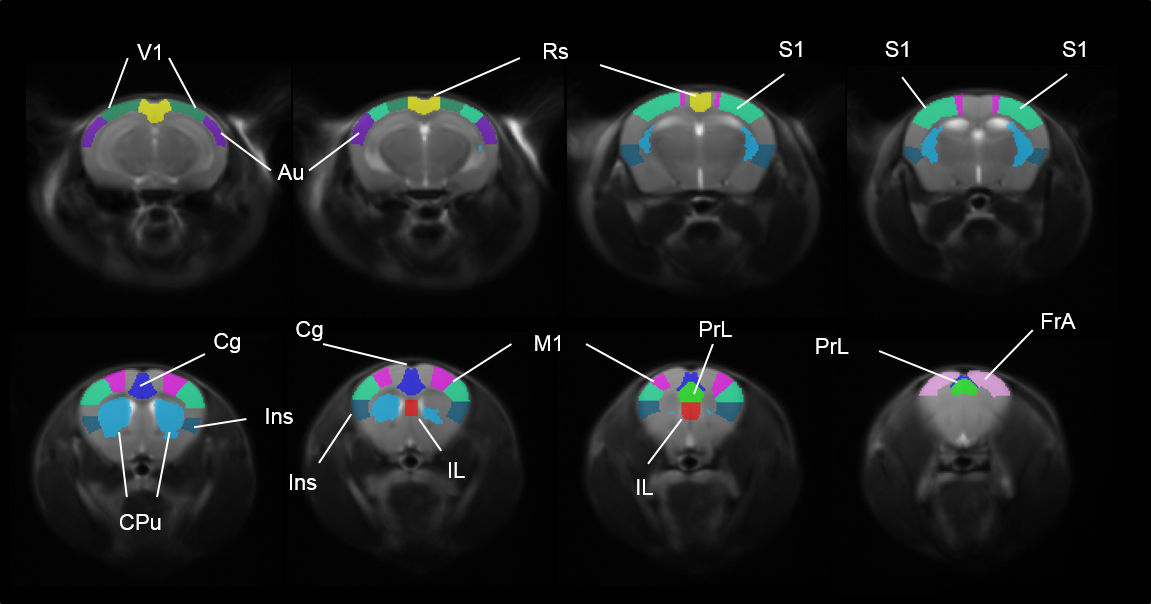
\includegraphics[scale=0.6]{figures/cntnap2_figure_s1.png}
    \decoRule
    \caption[Volumes of interest used in functional connectivity mappings.]{V1,
    primary visual cortex; Au, auditory cortex; Rs, retrosplenial cortex; S1,
    primary somatosensory cortex; Cg, cingulate cortex; CPu, caudate-putamen;
    Ins, insular cortex; IL, infra-limbic cortex; M1, primary motor cortex; PrL,
    prelimbic cortex; FrA, frontal association cortex.}
    \label{fig:cntnap2_figs1}
\end{figure}

Inter-group differences in the extension and intensity of long-range rsfMRI
correlation networks were mapped using seed-based approach as previously
described \parencite{sforazzini2016}. Small a priori seed regions of $3 \times 3
\times 1$ voxels were chosen to cover antero-posterior cortical networks and
representative heteromodal cortical structures (Fig.~\ref{fig:cntnap2_figs2}).
The mean time courses from the unilateral (medial, Rs, PrL) and bilateral seeds
(TeA, Pt, and vHC) were used as regressors for each voxel. Group level
differences in connectivity distributions were mapped using two-tailed Student’s
t-tests (p < 0.05 FWE cluster corrected with cluster-defining threshold of t24 >
2.06, p < 0.05, as implemented in FSL).

\begin{figure}[th] 
    \centering
    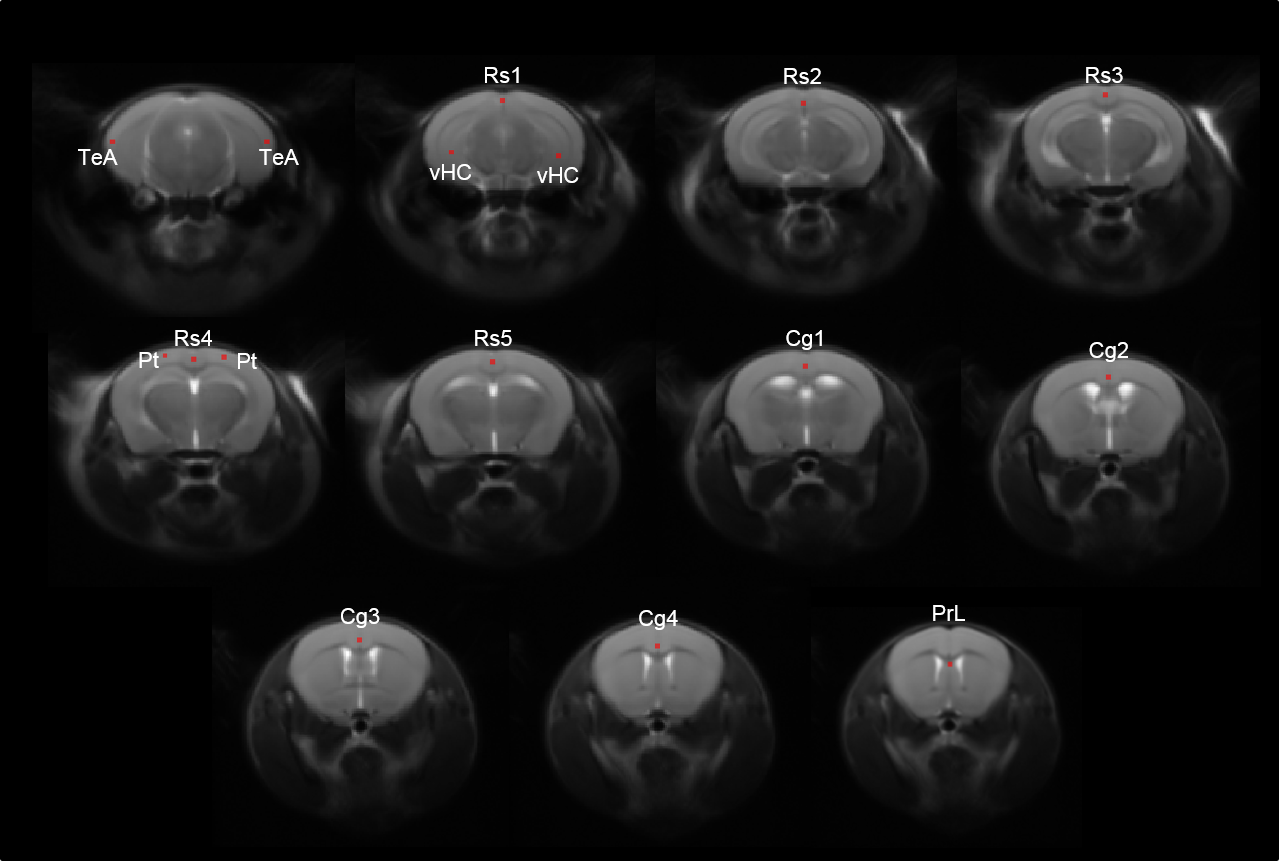
\includegraphics[scale=0.6]{figures/cntnap2_figure_s2.png}
    \decoRule
    \caption[Location of seeds used in mapping anteroposterior DMN
    connectivity.]{Location of seeds used in mapping anteroposterior DMN
    connectivity. TeA, temporal association cortex (bilateral); Rs,
    retrosplenial cortex; Cg, cingulate cortex; Pt, posterior parietal
    association cortex (bilateral); PrL, prelimbic cortex; vHC: ventral
    hippocampus.}
    \label{fig:cntnap2_figs2}
\end{figure}

Alterations in inter-hemispheric functional connectivity were assessed by
computing correlation coefficients of inter-hemispheric VOI pairs depicted in
Fig.~\ref{fig:cntnap2_figs1}. The statistical significance of inter-group
correlation strength in each VOI was assessed with a two-tailed Student’s t-test
(t24 > 2.06, p < 0.05) and corrected for multiple comparisons using a false
discovery rate q = 0.05 according to the Benjamini-Hochberg procedure.

Anteroposterior DMN connectivity was mapped by computing seed-to-VOI
correlations. Prelimbic and cingulate cortex were employed as prefrontal volumes
of interest. The location of seeds employed for mapping are indicated in
Fig.~\ref{fig:cntnap2_figs2}. The statistical significance of inter-group
effects was quantified using a two-way repeated-measures ANOVA, where seed
location and genotype were used as variables. 

\subsection{Diffusion MRI}

Ex vivo diffusion-weighted (DW) MRI was carried out on paraformaldehyde fixed
specimens as previously described (dodero2013). At the end of the rsfMRI
experiments, mice were transcardially perfused with 4% para-formaldehyde under
deep isoflurane anaesthesia. Brains were imaged inside intact skulls to avoid
post-extraction deformations. Each DW dataset was composed of 8
non-diffusion-weighted images and 81 different diffusion gradient-encoding
directions with $b=\SI{3000}{s/mm^2}$ ($\delta=\SI{6}{ms}$, $\Delta=13$ ms) acquired using an
EPI sequence with the following parameters: $\text{TR/TE}=13500/27.6$ \si{ms}, field of view
$1.68 \times 1.54$ \si{cm^2}, matrix $120 \times 110$, in-plane spatial resolution
$140 \times 140$ \si{\um^2}, 54 coronal slices, slice thickness \SI{280}{um}, number of
averages 20. Three mice were discarded from the analyses owing to the presence
of large susceptibility distortions in the DW images due to the presence of air
bubbles following imperfect perfusion procedure. As a result of this, the final
number of subjects per group was n = 13 and n = 10, for \textit{Cntnap2}$^{+/+}$ and
\textit{Cntnap2}$^{-/-}$, respectively.

\subsection{White-matter fibre tractography}

The DW datasets were first corrected for eddy current distortions
(FSL/eddy\_correct) and skull-stripped (\parencite{oguz2014}). The resulting
individual brain masks were manually corrected using ITK-SNAP
(\parencite{yushkevich2006}). Whole brain tractography was performed using
MRtrix3 \parencite{tournier2012} using constrained spherical deconvolution [lmax
= 8, \parencite{tournier2007}] and probabilistic tracking (iFOD2) with a FOD
amplitude cut-off of 0.2. For each dataset, the whole brain mask was used as a
seed, and a total of 100,000 streamlines were generated.

The corpus callosum and cingulum were selected as tracts of interest, given
their major cortico-cortical extension and direct involvement in
prefrontal-posterior connectivity \parencite{vogt2014}. The tracts were
virtually dissected with waypoint VOIs described in Fig.~\ref{fig:cntnap2_figs3}
using TrackVis (\url{http://www.trackvis.org/}). Inter-group differences in streamline
counts of the tracts were evaluated using a two-tailed Student’s t-test ($t_{21} >
2.08$, $p < 0.05$). To provide a visual assessment of fibre distribution across
groups, voxelwise parametric fibre density maps were generated using DiPy
\parencite{garyfallidis2014}, by determining for each voxel the number of
subjects in which at least one streamline of the fibre tract of interest passes
through the voxel. For visualization purposes, both the dissected tracts and
group fibre density maps were transformed to the Allen Mouse Common Coordinate
Framework, Version 3 (\url{http://www.brain-map.org/}).

\begin{figure}[th] 
    \centering
    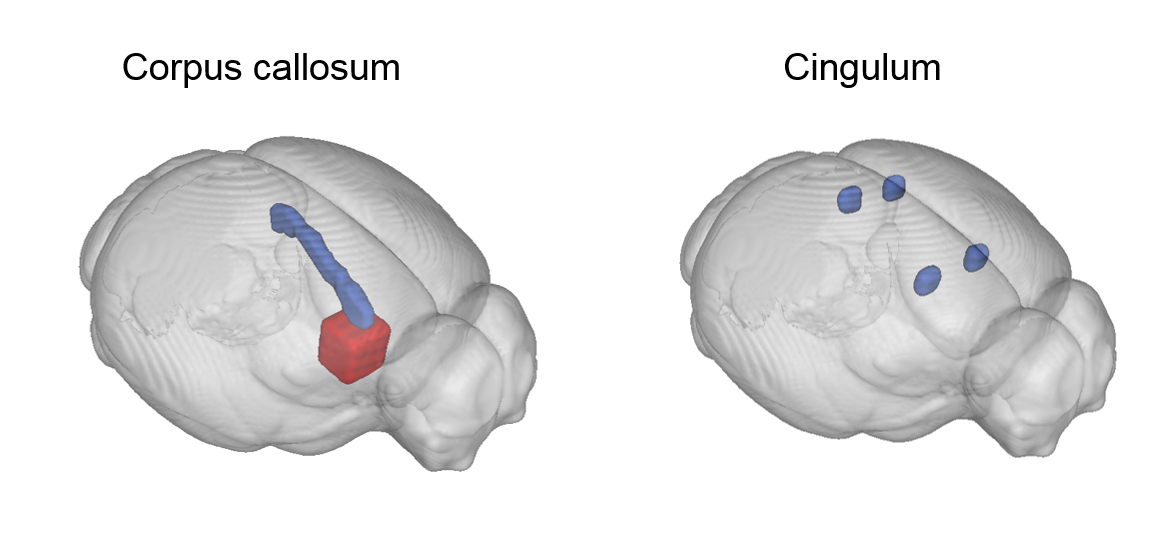
\includegraphics[scale=0.7]{figures/cntnap2_figure_s3.png}
    \decoRule
    \caption[Location of waypoint ROIs used for virtual dissection of
    corpus callosum and cingulum tracts from whole-brain white matter
    tractography.]{Location of waypoint ROIs used for virtual dissection of
    corpus callosum and cingulum tracts from whole-brain white matter
    tractography. Inclusion ROIs are indicated in blue, exclusion ROIs are
    indicated in red.}
    \label{fig:cntnap2_figs3}
\end{figure}

\subsection{Rabies virus production and injection}

Unpseudotyped recombinant SAD$\Delta$G-mCherry rabies virus (RV) was produced as
described by \textcite{osakada2013}. Briefly, B7GG packaging cells,
which express the rabies envelope G protein, were infected with unpseudotyped
SAD$\Delta$G-mCherry-RV, obtained by courtesy of Prof. Edward Callaway from the Salk
Institute. After five to six days, the virus was collected, filtrated with 0.45
$\mu m$ filter and concentrated by two rounds of ultracentrifugation. The titer of
the SAD$\Delta$G-mCherry-RV preparation was established by infecting Hek-293T cells
(ATCC cat no. CRL-11268) with tenfold serial dilution of viral stock, counting
mCherry expressing cells 3 days after infection. The titer was calculated as
2x1011 Infective Units (IU)/ml, and the stock was therefore considered suitable
for in vivo microinjection. Intracortical rabies virus injections were carried
out as previously described \parencite{sforazzini2016} in adult (12-16 week-old)
male \textit{Cntnap2}$^{-/-}$ and control \textit{Cntnap2}$^{+/+}$ littermates (n = 6, each group). To this
purpose, mice were deeply anesthetized with avertin (250 mg/kg) and firmly
stabilized on a stereotaxic apparatus (Stoelting Inc.). A micro drill (Cellpoint
Scientific Inc.) was used to drill holes through the skull. Injections were
performed with a Nanofil syringe mounted on an UltraMicroPump UMP3 with a four
channel Micro4 controller (World Precision Instruments), at a speed of 5 nl/s,
followed by a 5–10 minutes waiting period, to avoid backflow of viral solution
and unspecific labelling. One $\mu l$ of viral stock solution was injected
unilaterally in the left anterior prefrontal cortex using the following
coordinates for injections, expressed in mm from bregma: 1.42 from anterior to
posterior, 0.3 lateral, -1.6 deep \parencite{paxinos2004} 

\subsection{Quantification of retrogradely labelled cells}

RV-labelled cell quantification and histological analyses where carried out by
an operator (A.B.) blind to genotype. After 7 days from viral injection, the
animals were transcardially perfused with 4 \% paraformaldehyde (PFA), brains
were dissected, post-fixed over night at $4\degree$C and vibratome-cut (Leica
Microsystems).  RV-infected cells were detected by means of immunohistochemistry
performed on every other 100 $\mu m$ thick coronal section, using rabbit anti-red
fluorescent protein (RFP) primary antibody (1:500, AbCam), and goat anti-rabbit
HRP secondary antibody (1:500, Jackson ImmunoResearch), followed by 3-3’
diaminobenzidine tetrahydrochloride (DAB, Sigma Aldrich) staining. Imaging was
performed with MacroFluo microscope (Leica). Each picture was then superimposed
onto the corresponding Paxinos Atlas table \parencite{paxinos2004}, and cell
bodies were plotted according to their anatomical localization. The cells were
then assigned to their corresponding brain regions, and final region-based cell
population counts were expressed as fraction of the total amount of labelled
cells.

\subsection{Histological and immunohistochemical analysis of white matter}

To histologically assess the presence of microstructural white matter
alterations, we examined immunofluorescence-enhanced coronal brain sections
covering anterior callosal regions from adult (12 week-old) male \textit{Cntnap2}$^{-/-}$ and
control \textit{Cntnap2}$^{+/+}$ littermates (n = 5, each group) after incubation with rat
anti-myelin basic protein (MBP) primary antibody (1:1000, AbCam), followed by
donkey anti-rat 594 secondary antibody (1:500, Thermo scientific). We also
quantified MBP levels as previously described \parencite{mottershead2003,
richetto2017}.  Briefly, three representative random images in anterior callosal
regions characterized by parallel or transversal fiber extension with respect to
the image plane (corpus callosum and forceps minor of the corpus callosum,
respectively) were acquired on a Nikon A1 confocal system, equipped with 561
laser diode and appropriate filter for Texas Red fluorophore. Z-stack images
(1.5 $\mu m$ thick) were acquired using an oil-immersion 60x plan-apochromat
objective at 1024x1024 pixel resolution. Callosal image fields were also
qualitatively inspected for the presence of inter-group differences in white
matter organization or reduced neuronal packing/density. MBP content was
empirically quantified by summing MBP-immunoreactive areas expressed as number
of pixels whose values were above the background threshold, calculated as pixel
intensity values in areas with no detectable immunostaining, such as cell nuclei
or MBP-devoid background.

\section{Results}

\subsection{Reduced local and long-range connectivity in fronto-cortical regions
of \textit{Cntnap2}$^{-/-}$ mice}

To obtain an unbiased mapping of genotype-dependent differences in functional
connectivity, we implemented recently developed aggregative metrics for local
and long-range functional connectivity. This analysis revealed foci of
significantly reduced local and long-range connectivity in \textit{Cntnap2}$^{-/-}$ mutants
with respect to wild-type control subjects (t-test, p < 0.05 FWE
cluster-corrected, with cluster-defining threshold of t24 > 2.06, p < 0.05;
Fig.~\ref{fig:cntnap2_fig01}) encompassing prefrontal (prelimbic and cingulate)
and retrosplenial cortices.  These same brain regions have been classified both
in mice and in humans as “high strength” functional connectivity hubs
\parencite{buckner2009, cole2010, liska2015}, and as such are thought to play a
key integrative role in distributed functional networks. Local connectivity
reductions appeared to be more widespread than corresponding long-range
connectivity deficits (Fig.~\ref{fig:cntnap2_fig01}a, c), encompassing
involvement of supplementary motor areas surrounding cingulate cortex. The
observed local and long-range connectivity reductions were statistically
significant also when integrated over a large volume of interest encompassing
the whole cingulate cortex (local connectivity: Cg, t-test, t24 = 3.11, p =
0.005, Fig.~\ref{fig:cntnap2_fig01}b; long-range connectivity: Cg, t-test, t24 =
2.26, p = 0.03, Fig.~\ref{fig:cntnap2_fig01}d). 

\begin{figure}[th] 
    \centering
    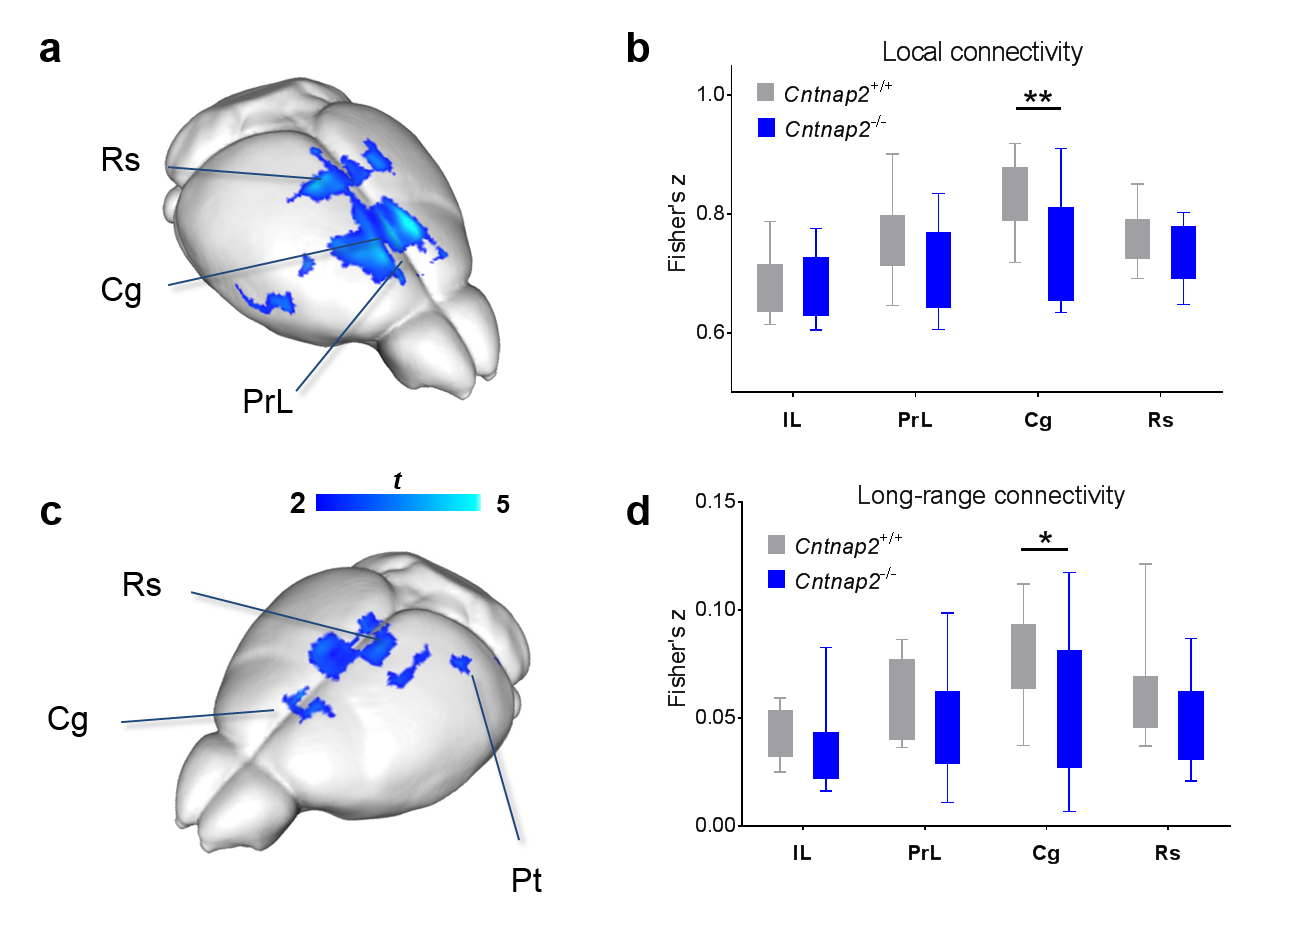
\includegraphics[scale=0.6]{figures/cntnap2_figure_01.png}
    \decoRule
    \caption[Reduced local and long-range connectivity in \textit{Cntnap2}$^{-/-}$
    mutants.]{Reduced local and long-range connectivity in \textit{Cntnap2}$^{-/-}$ mutants.
    (\textbf{a}) Foci of reduced local connectivity in \textit{Cntnap2}$^{-/-}$ vs. control
    \textit{Cntnap2}$^{+/+}$ littermates (t-test; t24 > 2.06, p < 0.05; cluster corrected with
    cluster-level p < 0.05). (\textbf{b}) Mean local connectivity in regions of
    interest (t-test; Cg: t24 = 3.11, p = 0.005). (\textbf{c}) Foci of reduced
    long-range connectivity in \textit{Cntnap2}$^{-/-}$ vs. control \textit{Cntnap2}$^{+/+}$ littermates
    (t-test; p < 0.05 FWE cluster-corrected, with cluster-defining threshold of
    t24 > 2.06, p < 0.05). (\textbf{d}) Mean long-range connectivity in regions
    of interest (t-test; Cg: t24 = 2.26, p = 0.03). IL, infra-limbic cortex;
    PrL, prelimbic cortex, Cg, cingulate cortex; Rs, retrosplenial cortex, * p <
    0.05, **p < 0.01.}
    \label{fig:cntnap2_fig01}
\end{figure}


\subsection{Long-range connectivity impairments in \textit{Cntnap2}$^{-/-}$ mice affect
heteromodal cortical regions and the DMN}

To identify regional targets of the observed long-range connectivity deficits,
we probed rsfMRI networks previously shown to involve prefrontal, cingulate and
retrosplenial regions \parencite{sforazzini2014, gozzi2016}. Seed-based mapping
of retrosplenial and anterior cingulate/prelimbic cortex highlighted foci of
reciprocal long-range hypoconnectivity along the midline brain axis in
\textit{Cntnap2}$^{-/-}$ mutants (t-test, p < 0.05 FWE cluster-corrected, with
cluster-defining threshold of t24 > 2.06, p < 0.05;
Fig.~\ref{fig:cntnap2_fig02}a, b). We also probed connectivity of putative
lateral components of the rodent DMN such as the posterior parietal and temporal
association/auditory cortices, and postero-ventral hippocampus
\parencite{gozzi2016}. Parietal cortical mapping revealed foci of reduced local
and long-range (middle cingulate) connectivity in \textit{Cntnap2}$^{-/-}$ mice (t-test, p <
0.05 FWE cluster-corrected, with cluster-defining threshold of t24 > 2.06, p <
0.05; Fig.~\ref{fig:cntnap2_fig02}c). In the same animals, temporal association
areas appeared to be widely hypo-connected to retrosplenial, cingulate and
prefrontal regions (t-test, p < 0.05 FWE cluster-corrected, with
cluster-defining threshold of t24 > 2.06, p < 0.05;
Fig.~\ref{fig:cntnap2_fig02}d). We also observed foci of long-range
hypo-connectivity between ventral hippocampal and ventral prefrontal
(infralimbic) regions (t-test, p < 0.05 FWE cluster-corrected, with
cluster-defining threshold of t24 > 2.06, p < 0.05;
Fig.~\ref{fig:cntnap2_fig02}e). Inter-hemispheric connectivity in subcortical or
motor-sensory networks appeared to be overall largely preserved. A reduction in
inter-hemispheric connectivity was observed in primary motor areas and visual
cortex when quantified in anatomical volumes of interest
(Fig.~\ref{fig:cntnap2_figs4}), although the effect did not survive false
discovery rate correction.

\begin{figure}[th] 
    \centering
    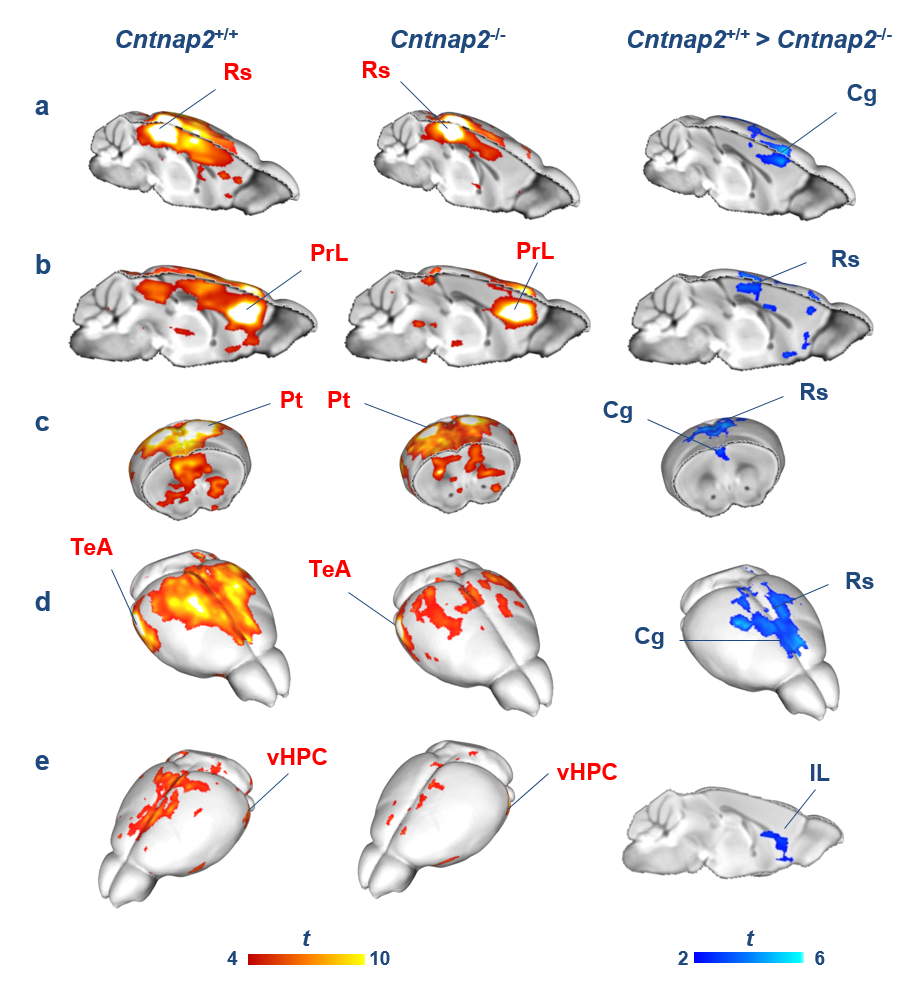
\includegraphics[scale=0.7]{figures/cntnap2_figure_02.png}
    \decoRule
    \caption[Reduced long-range connectivity in \textit{Cntnap2}$^{-/-}$ mice.]{Reduced
    long-range connectivity in \textit{Cntnap2}$^{-/-}$ mice. (\textbf{a}-\textbf{e})
    Seed-correlation mapping highlighted convergent reduced connectivity between
    long-range cortical and subcortical regions and cingulate-prefrontal areas.
    Red/yellow shows areas with significant correlation with seed regions
    indicated in red (one-sample t-test, p < 0.05 FWE cluster corrected with
    cluster-defining threshold of t12 > 2.18, p < 0.05). Blue indicates foci of
    reduced connectivity in \textit{Cntnap2}$^{-/-}$ mutants with respect to control mice
    (t-test, p < 0.05 FWE cluster corrected with cluster-defining threshold of
    t24 > 2.06, p < 0.05).  Rs, retrosplenial cortex; IL, infra-limbic cortex;
    PrL, prelimbic cortex; Cg, cingulate cortex; Rs, retrosplenial cortex; vHPC,
    ventral hippocampus; Au/TeA, auditory/temporal association cortices; Pt,
    parietal cortex.}
    \label{fig:cntnap2_fig02}
\end{figure}

\begin{figure}[th] 
    \centering
    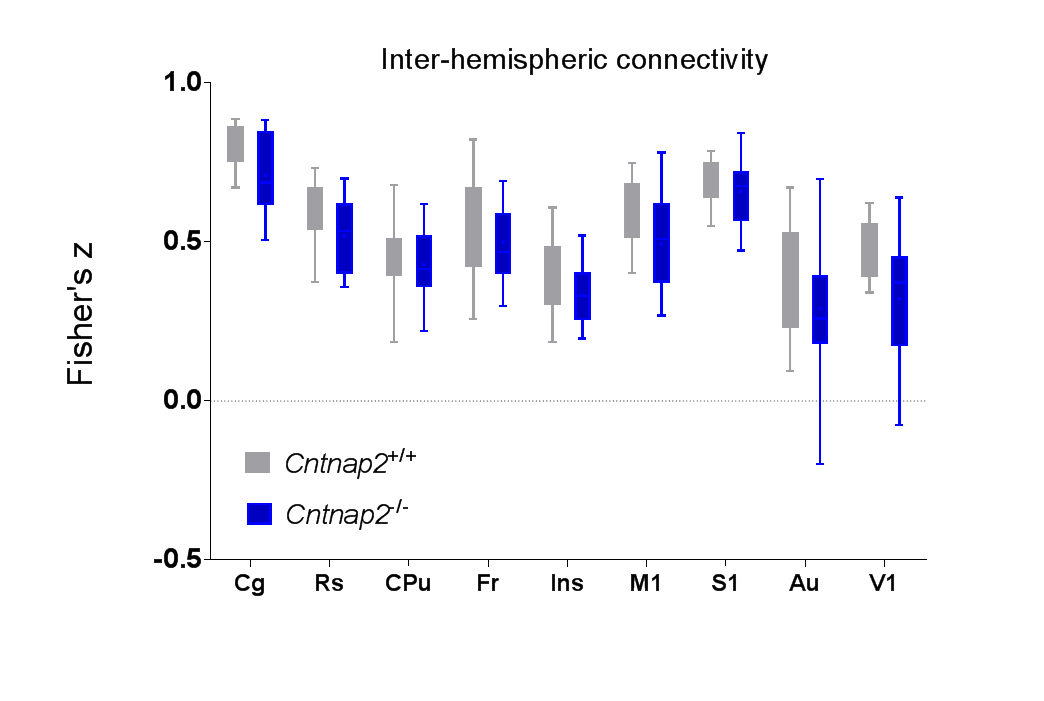
\includegraphics[scale=0.7]{figures/cntnap2_figure_s4.png}
    \decoRule
    \caption[Largely preserved inter-hemispheric connectivity in \textit{Cntnap2}$^{-/-}$
    mutants and control mice.]{Largely preserved inter-hemispheric connectivity
    in \textit{Cntnap2}$^{-/-}$ mutants and control mice. Correlation coefficients were
    calculated between time courses extracted from VOIs depicted in
    Fig.~\ref{fig:cntnap2_figs1} and the resulting r-scores were transformed to
    z-scores using Fisher’s r-to-z transform. None of these comparisons
    survived a false discovery rate correction at q = 0.05. }
    \label{fig:cntnap2_figs4}
\end{figure}

Importantly, no genotype-dependent differences in anaesthesia sensitivity were
detected as seen with mean arterial blood pressure mapping (t-test, t24 = 0.17,
p = 0.87; Fig.~\ref{fig:cntnap2_figs5}a) and amplitude of cortical BOLD signal
fluctuations (t-test, t24 = 0.72, p = 0.48; Fig.~\ref{fig:cntnap2_figs5}b), two
independent readouts previously shown to be linearly correlated with anaesthesia
depth \parencite{steffey2003, liu2011}.  Together with the observation of
region-dependent alterations, as opposed to the global reduction described with
increased anaesthesia dosing \parencite{nasrallah2014}, these findings strongly
argue against a confounding contribution of anaesthesia to the observed
hypo-connectivity. 

\begin{figure}[th] 
    \centering
    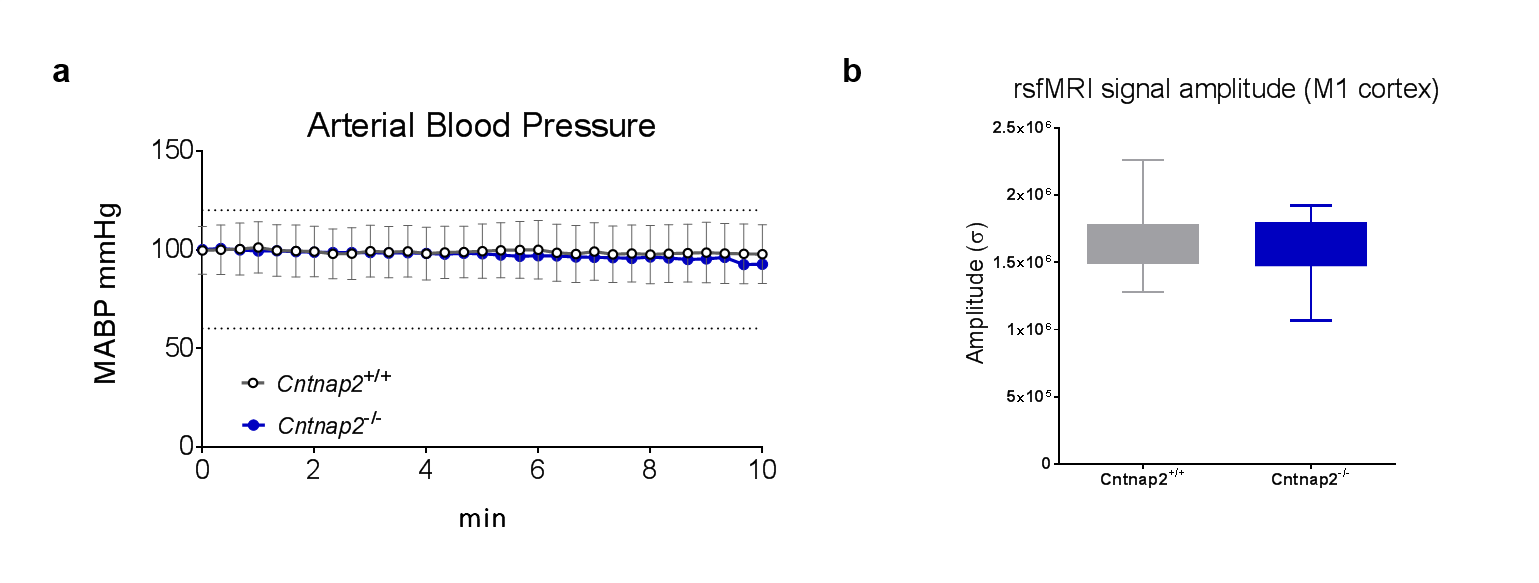
\includegraphics[scale=0.55]{figures/cntnap2_figure_s5.png}
    \decoRule
    \caption[No genotype-dependent differences in anaesthesia sensitivity in
    \textit{Cntnap2}$^{-/-}$ mice.]{No genotype-dependent differences in anaesthesia
    sensitivity were detected as seen with mean arterial blood pressure mapping
    (t-test, t24 = 0.17, p = 0.87; a) and amplitude of cortical BOLD signal
    fluctuations in primary motor cortex (t-test, t24 = 0.72, p = 0.48; b). M1,
    primary motor cortex.}
    \label{fig:cntnap2_figs5}
\end{figure}

\subsection{Hypoconnectivity in the mouse DMN is associated with impaired social
behaviour}

Recent human imaging studies in socially-impaired patients have revealed a
putative association between long-range DMN hypo-connectivity and social
competence \parencite{schreiner2014}. Based on these findings, we hypothesized
that reduced long-range DMN connectivity in \textit{Cntnap2}$^{-/-}$ mice could be associated
with impaired social behaviour. To test this hypothesis, we first corroborated
DMN hypoconnectivity by quantifying functional connectivity along the dorsal
midline axis of this network (anterior/middle cingulate cortex and
retrosplenial cortex) using multiple seed-to-VOI measurements
(Fig.~\ref{fig:cntnap2_fig03}). A clear dysconnection between posterior
(retrosplenial) and middle/anterior portions of the DMN (cingulate, prelimbic
cortex) was apparent (retrosplenial to cingulate cortex: two-way
repeated-measures ANOVA, genotype effect, F1,24 = 5.76, p = 0.02,
Fig.~\ref{fig:cntnap2_fig03}a; retrosplenial-cingulate to prelimbic: two-way
repeated-measures ANOVA, genotype effect, F1,24 = 6.82, p = 0.02,
Fig.~\ref{fig:cntnap2_fig03}b). 

\begin{figure}[th] 
    \centering
    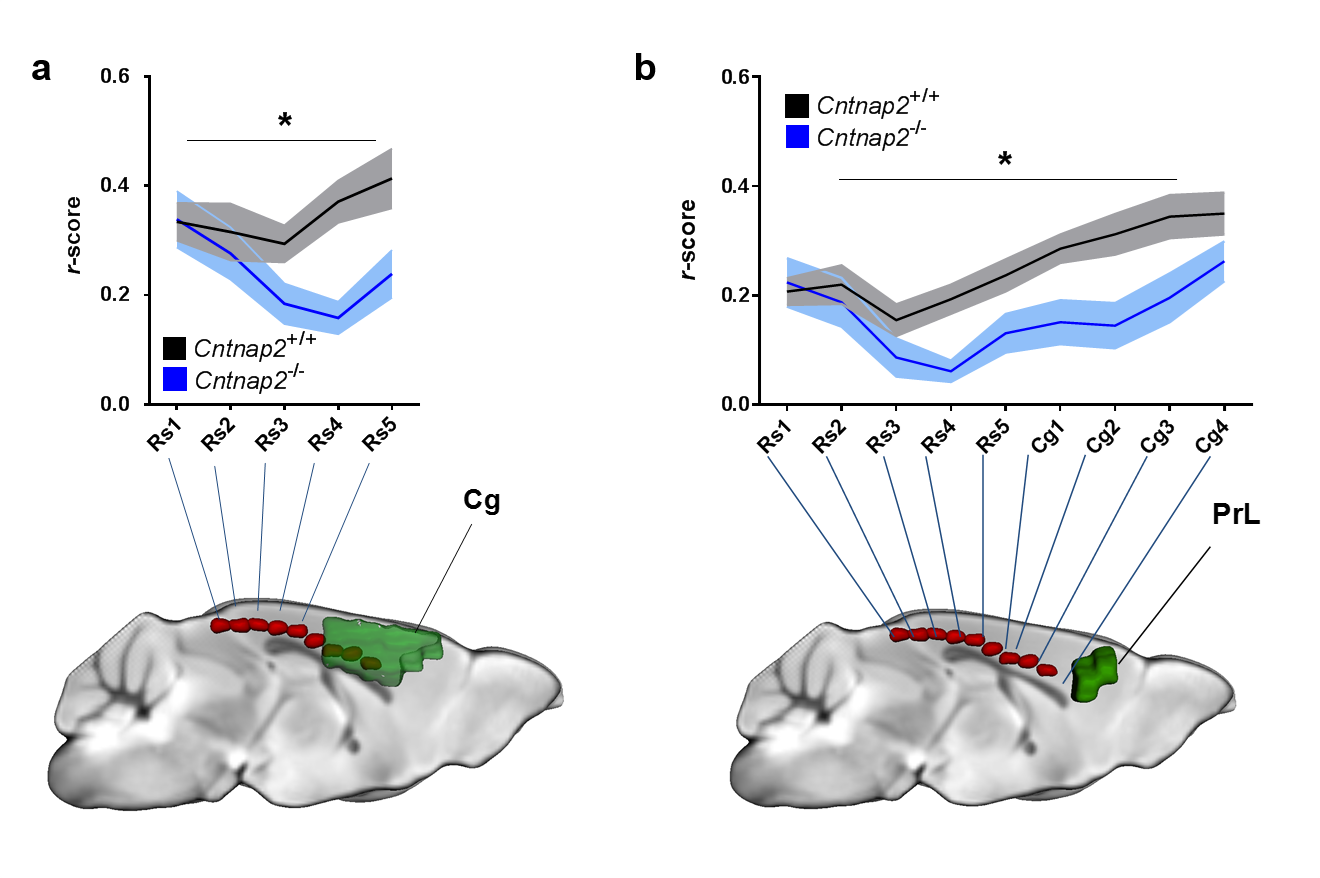
\includegraphics[scale=0.6]{figures/cntnap2_figure_03.png}
    \decoRule
    \caption[Fronto-posterior hypoconnectivity in \textit{Cntnap2}$^{-/-}$
    mice.]{Fronto-posterior hypoconnectivity in \textit{Cntnap2}$^{-/-}$ mice. (\textbf{a})
    Connectivity profile between a series of retrosplenial seeds (Rs, red) and
    the cingulate cortex (Cg, green) (two-way repeated-measures ANOVA, genotype
    effect, F1,24 = 5.76, p = 0.02). (\textbf{b}) Connectivity profile between a
    series of retrosplenial/cingulate seeds (Rs, Cg, red) and the prelimbic
    cortex (PrL, green) (two-way repeated-measures ANOVA, genotype effect, F1,24
    = 6.82, p = 0.02). * p < 0.05.}
    \label{fig:cntnap2_fig03}
\end{figure}

We then measured social behaviour in adult \textit{Cntnap2}$^{-/-}$ and \textit{Cntnap2}$^{+/+}$ control
mice in a male-female interaction test, and correlated the measured social
scores with DMN hypoconnectivity measures. Consistent with previous reports
\parencite{penagarikano2011}, behavioural testing revealed significantly
impaired social interest (total sniffing, duration: t-test, t24 = 2.29, p =
0.03, Fig.~\ref{fig:cntnap2_fig04}a; social investigation, duration: t-test, t24
= 2.43, p = 0.02, Fig.~\ref{fig:cntnap2_fig04}c) and increased non-social
behaviour (wall-rearing, frequency: t-test, t24 = 3.09, p = 0.01;
Fig.~\ref{fig:cntnap2_figs6}a) in \textit{Cntnap2}$^{-/-}$ mutants compared to \textit{Cntnap2}$^{+/+}$
control littermates. Hypo-connectivity in key DMN components
(retrosplenial-cingulate cortex) was significantly associated with reduced
social behaviour (total sniffing, duration: r = 0.42, p = 0.03, n = 26, R2 =
0.17, Fig.~\ref{fig:cntnap2_fig04}b; social investigation, duration: r = 0.40, p
= 0.04, n = 26, R2 = 0.16, Fig.~\ref{fig:cntnap2_fig04}d) and increased
non-social behaviour (wall rearing, frequency: r = -0.45, p = 0.02, n = 26, R2 =
0.21; Fig.~\ref{fig:cntnap2_figs6}b). These findings highlight a correlation
between fronto-posterior connectivity and social behaviour, suggesting that
impaired functional couplings produced by mutations in \textit{Cntnap2} could reverberate
to affect complex behavioural traits such as sociability and social exploration.

\begin{figure}[th] 
    \centering
    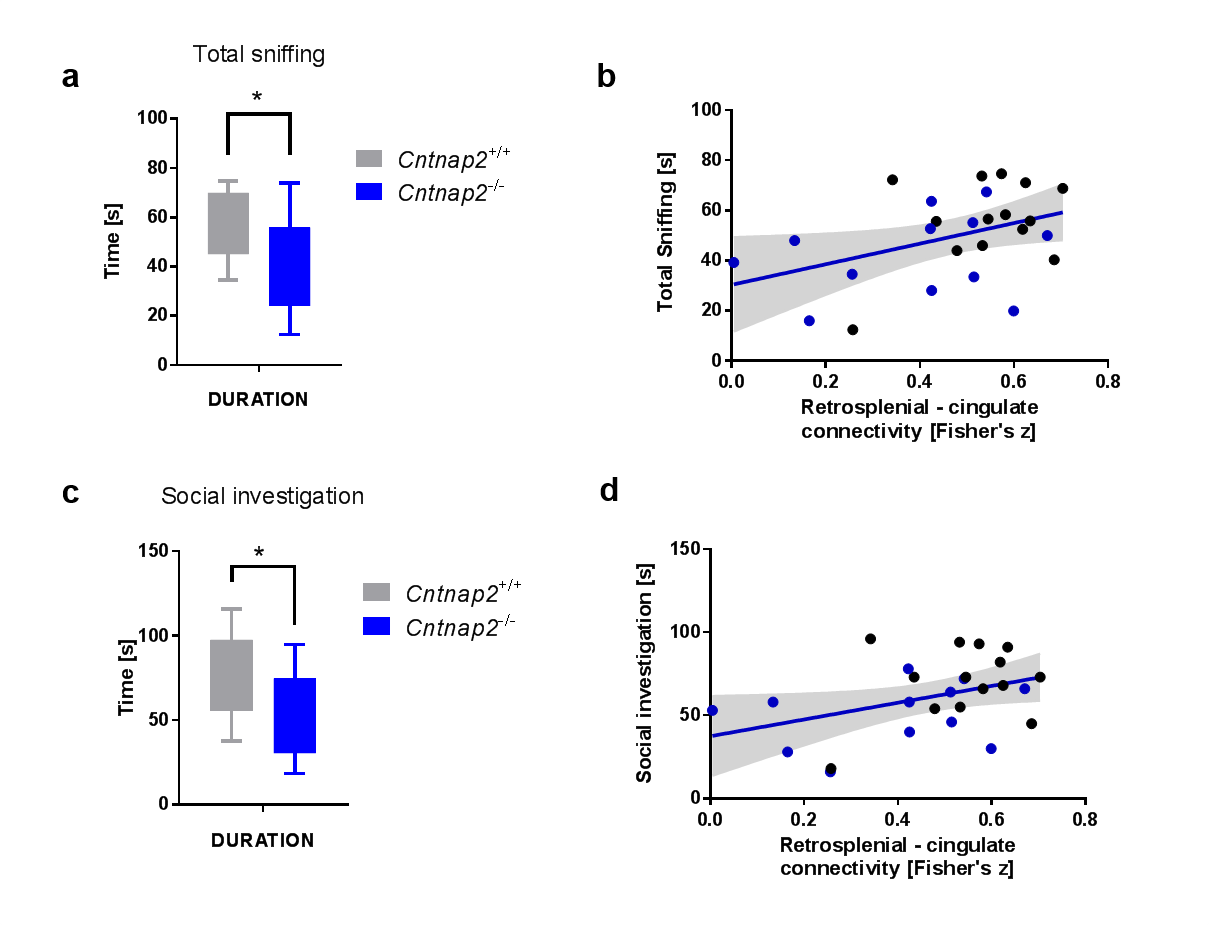
\includegraphics[scale=0.7]{figures/cntnap2_figure_04.png}
    \decoRule
    \caption[Fronto-posterior connectivity is correlated with social
    behaviour.]{Fronto-posterior connectivity is correlated with social
    behaviour.  (\textbf{a}) Social behaviour as measured by total sniffing
    duration (t-test, t24 = 2.29, p = 0.03). (\textbf{b}) Association between
    retrosplenial-cingulate connectivity (VOI to VOI) and total sniffing
    duration (r = 0.42, p = 0.03, n = 26, R2 = 0.17). (\textbf{c}) Social
    behaviour as measured by the duration of social investigation (t-test, t24 =
    2.43, p = 0.02). (\textbf{d}) Association between retrosplenial-cingulate
    connectivity (VOI-to-VOI) and the duration of social investigation (r =
    0.40, p = 0.04, n = 26, R2 = 0.16). * p < 0.05.}
    \label{fig:cntnap2_fig04}
\end{figure}

\begin{figure}[th] 
    \centering
    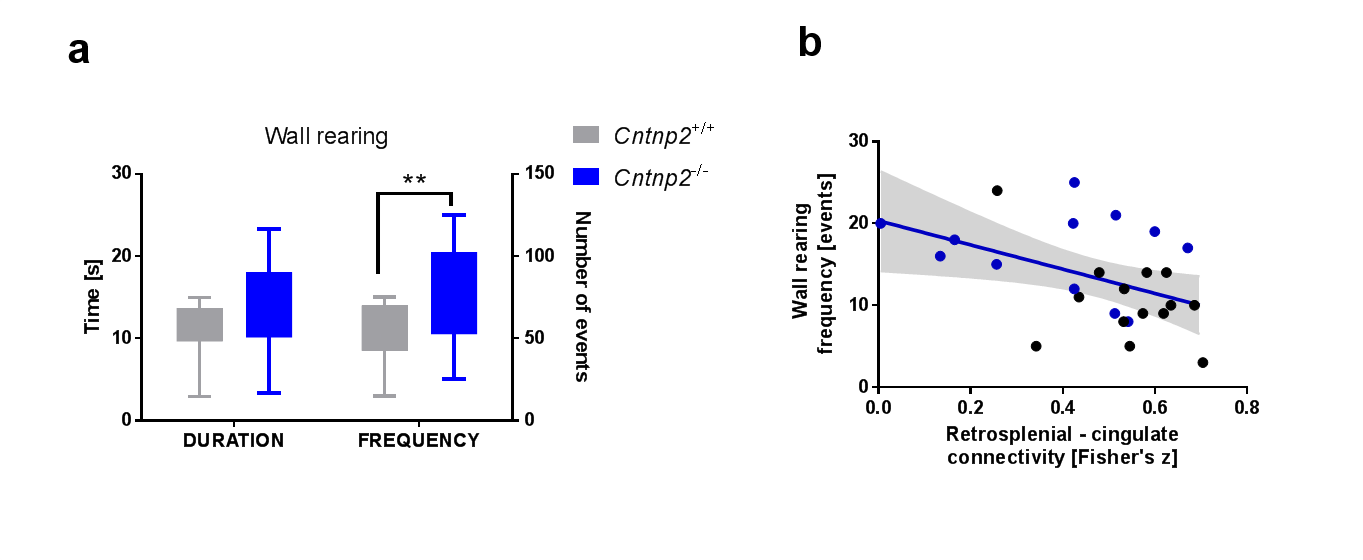
\includegraphics[scale=0.65]{figures/cntnap2_figure_s6.png}
    \decoRule
    \caption[Increased non-social behaviour in \textit{Cntnap2}$^{-/-}$ mutants compared to
    control littermates.]{Increased non-social behaviour in \textit{Cntnap2}$^{-/-}$ mutants
    compared to control littermates. (\textbf{a}) Non-social behaviour as
    measured by the duration and frequency of rearing up against the wall of the
    home-cage (frequency: t-test, t24 = 3.09, p = 0.01). (\textbf{b}) An inverse
    association between non-social behaviour and connectivity between
    retrosplenial and cingulate cortices (wall rearing, frequency: r = -0.45, p
    = 0.02, n = 26, R2 = 0.21). * p < 0.05, ** p < 0.01.}
    \label{fig:cntnap2_figs6}
\end{figure}

\subsection{Macroscale cortico-cortical white matter connectivity is preserved
in \textit{Cntnap2}$^{-/-}$ mice}

To probe a role of macroscale anatomical connectivity alterations on the
observed functional decoupling in \textit{Cntnap2}$^{-/-}$, we performed tractography analysis
of the corpus callosum and cingulum, two major white matter tracts characterised
by extensive cortico-cortical antero-posterior extension
(Fig.~\ref{fig:cntnap2_fig05}a). These white matter tracts appeared to be
largely typical in mutant and control mice as seen with group-level fibre
density maps (Fig.~\ref{fig:cntnap2_fig05}b); in keeping with this, we did not
observe statistically significant differences in the number of streamlines
between \textit{Cntnap2}$^{-/-}$ mutants and controls (cingulum: t-test, t21 = 1.25, p = 0.23;
corpus callosum: t-test, t21 = 1.21, p = 0.24; Fig.~\ref{fig:cntnap2_figs7}).
These results argue against a contribution of gross macroscale white matter
alterations to the observed functional connectivity impairments.

\begin{figure}[th] 
    \centering
    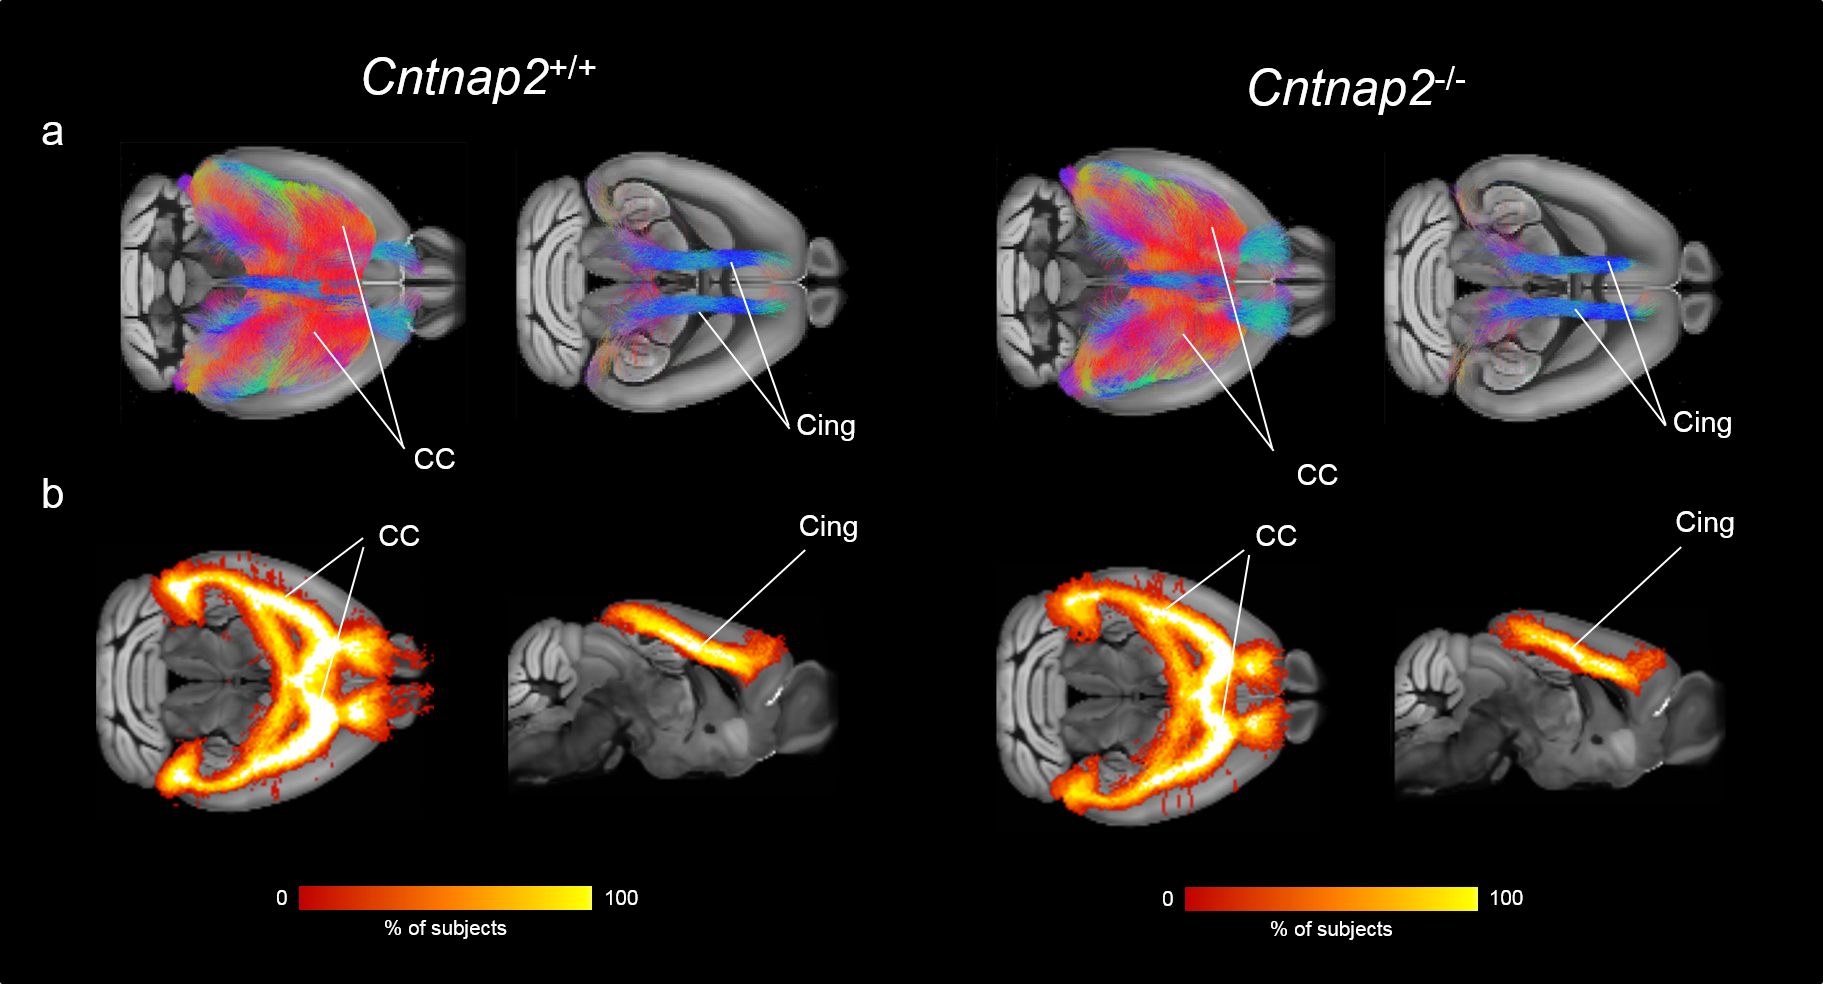
\includegraphics[scale=0.45]{figures/cntnap2_figure_05.png}
    \decoRule
    \caption[Preserved cortico-cortical white matter organization
    in \textit{Cntnap2}$^{-/-}$ mutants.]{Preserved cortico-cortical white matter organization
    in \textit{Cntnap2}$^{-/-}$ mutants. (\textbf{a}) Corpus callosum and cingulum tracts virtually
    dissected in two representative subjects (\textit{Cntnap2}$^{+/+}$ left, \textit{Cntnap2}$^{-/-}$
    right), (\textbf{b}) Fractional group fibre density maps for corpus callosum and
    cingulum tracts (\textit{Cntnap2}$^{+/+}$ left, \textit{Cntnap2}$^{-/-}$, right).}
    \label{fig:cntnap2_fig05}
\end{figure}

\begin{figure}[th] 
    \centering
    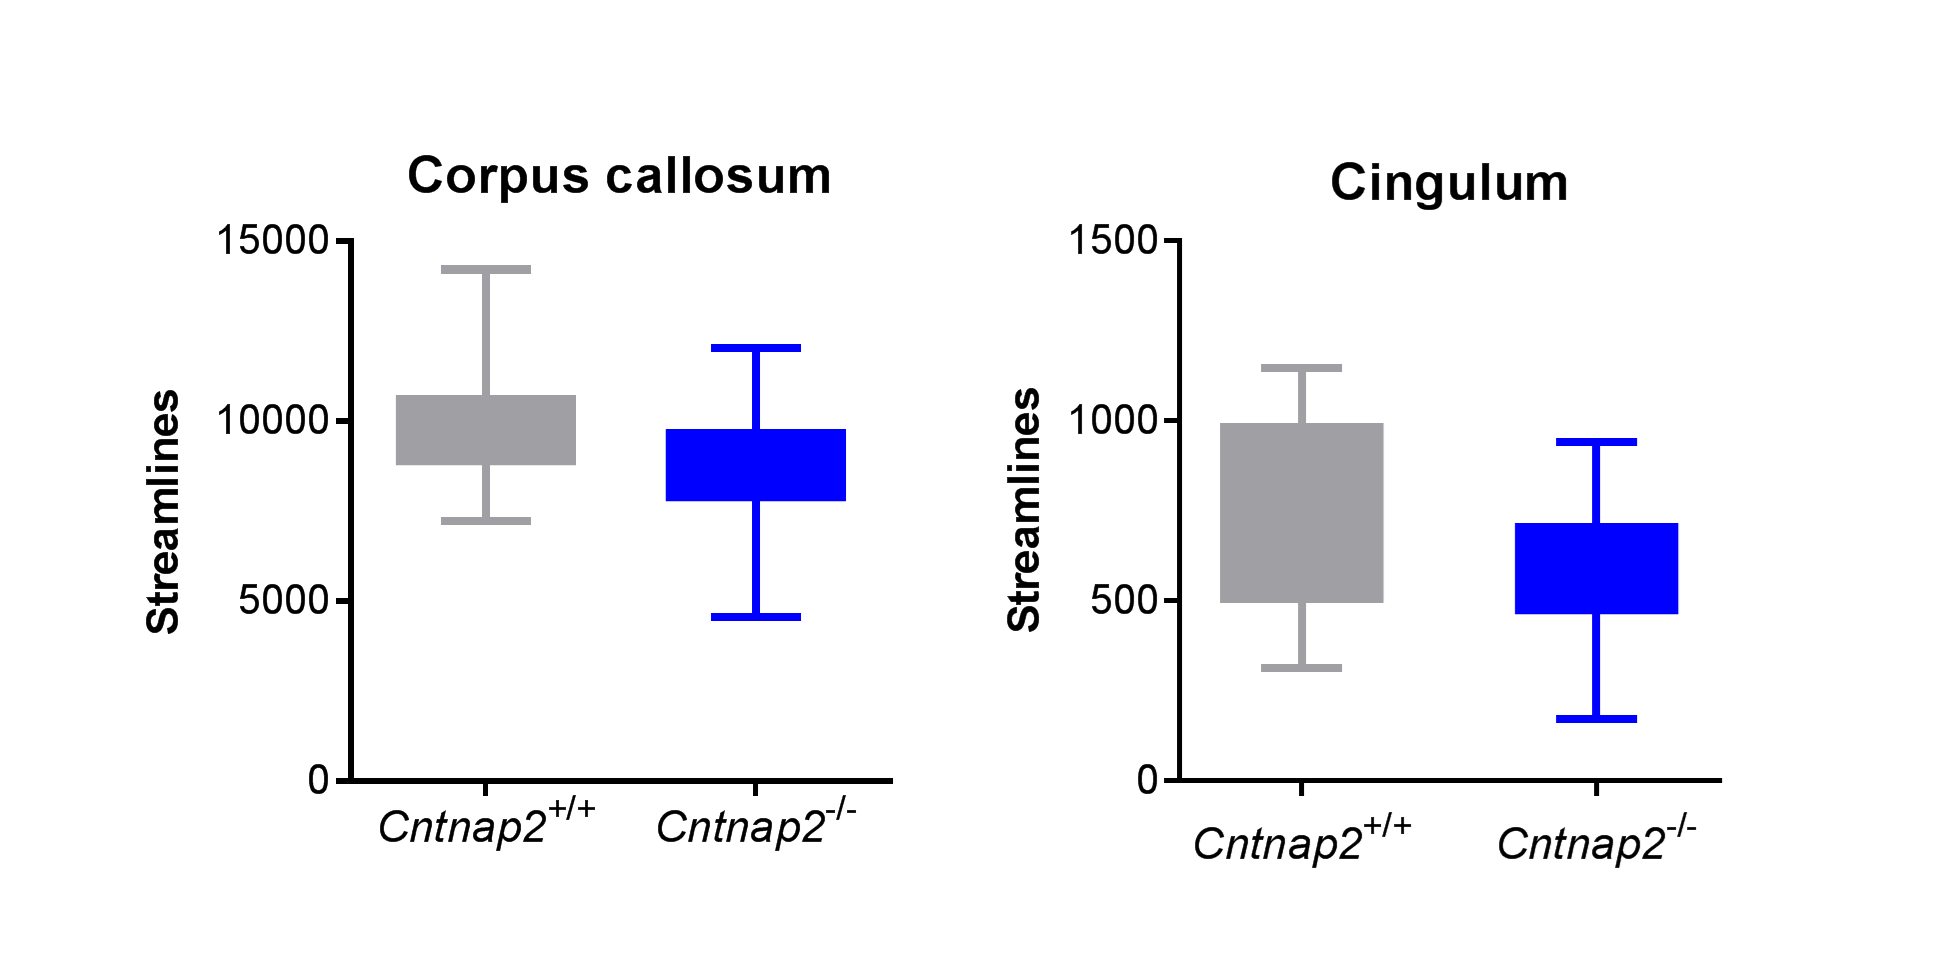
\includegraphics[scale=0.4]{figures/cntnap2_figure_s7.png}
    \decoRule
    \caption[White-matter tractography-based streamline counts.]{White-matter
    tractography-based streamline counts.  Numbers of streamlines in corpus
    callosum and cingulum showed no significant differences between the
    \textit{Cntnap2}$^{-/-}$ and control littermates (cingulum: t-test, t21 = 1.25, p = 0.23;
    corpus callosum: t-test, t21 = 1.21, p = 0.24).}
    \label{fig:cntnap2_figs7}
\end{figure}

\subsection{Reduced prefrontal-projecting neuronal clusters in cingulate cortex
of \textit{Cntnap2}$^{-/-}$ mice}

Although macroscale cortico-cortical connectivity appeared to be normal in
\textit{Cntnap2}$^{-/-}$ mutants, the possibility exists that finer-scale miswiring,
undetectable by tractography, may contribute to the mapped functional
connectivity alterations. To probe this hypothesis, we carried out monosynaptic
retrograde tracing of the left prefrontal cortex [prelimbic/anterior cingulate
cortex area 1, corresponding to Brodmann area 24Ab, \parencite{vogt2014}] and
quantified the number of retrogradely labelled cells in representative volumes
of interest in mutant and control littermate mice
(Fig.~\ref{fig:cntnap2_fig06}a). The anatomical distribution of retrogradely
labelled neurons in both genotypes was in keeping with previously published
rodent studies \parencite{hoover2007} and encompassed several key anatomical
substrates considered to be part of the rodent DMN \parencite{gozzi2016}.
Notably, regional quantification of the relative fraction of labelled cells
revealed reduced frequency of prefrontal-projecting neurons in the cingulate
cortex of \textit{Cntnap2}$^{-/-}$ mutants (Cg: t-test, t10 = 3.90, p = 0.003, FDR-corrected p
= 0.04; Fig.~\ref{fig:cntnap2_fig06}b, c). Importantly, no genotype-dependent
significant difference in the number of prefrontal projecting neurons was
observed in any of the other cortical or subcortical regions examined
(Fig.~\ref{fig:cntnap2_fig06}c).

\begin{figure}[th] 
    \centering
    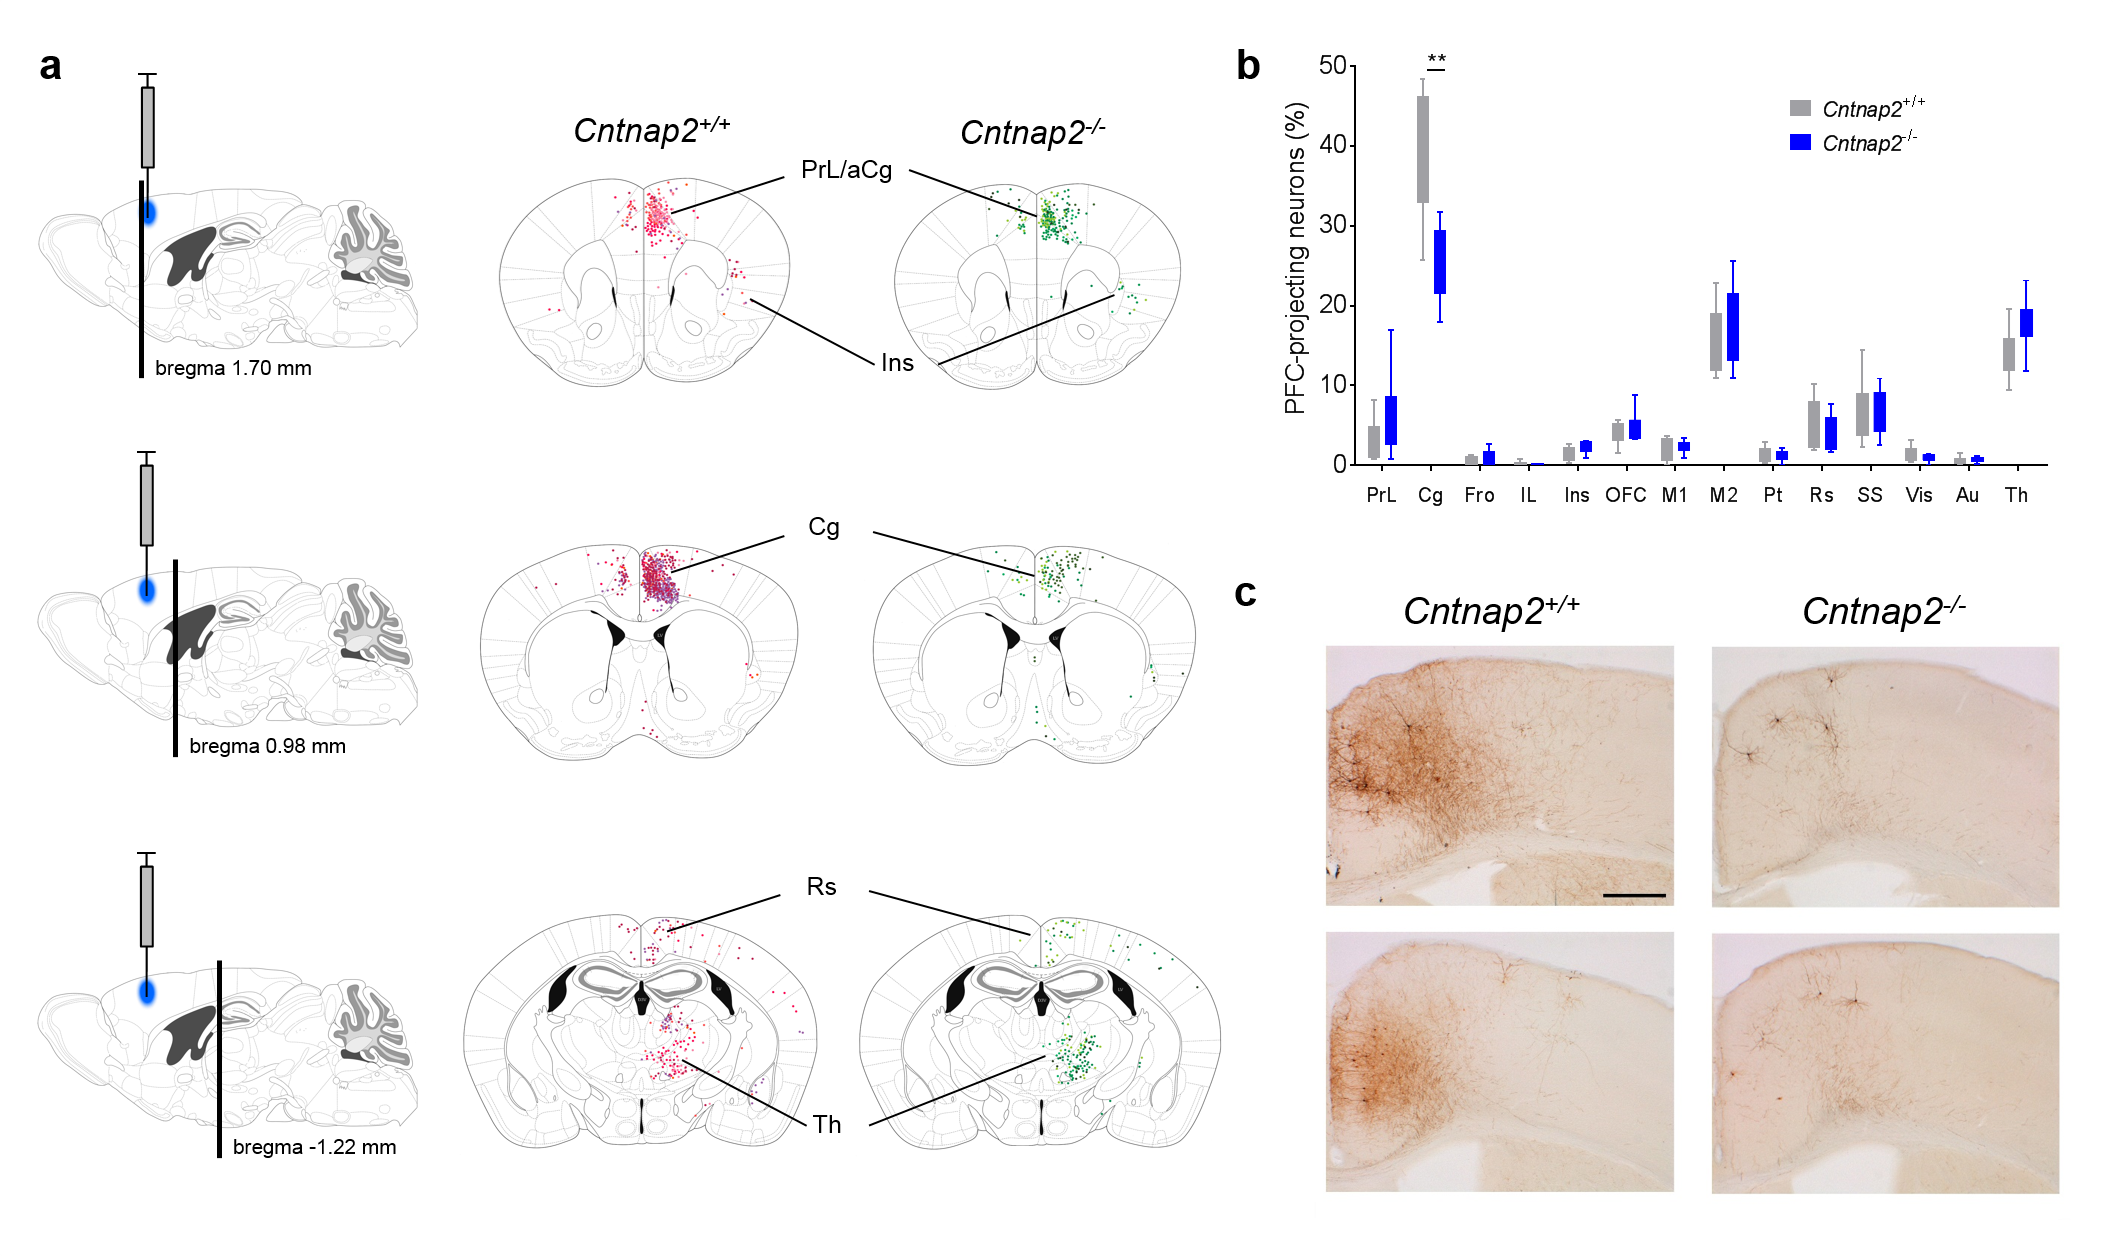
\includegraphics[scale=0.4]{figures/cntnap2_figure_06.png}
    \decoRule
    \caption[Reduced frequency of cingulate-prefrontal projecting neurons in
    \textit{Cntnap2}$^{-/-}$ mice.]{Reduced frequency of cingulate-prefrontal projecting
    neurons in \textit{Cntnap2}$^{-/-}$ mice. (\textbf{a}) Locations of retrogradely labelled
    cells superimposed on the corresponding Paxinos Atlas coronal tables.
    Injection location is indicated in blue on the sagittal tables. (\textbf{b})
    Regional quantification of the relative regional number (frequency) of
    retrogradely labelled cells (t-test; Cg: t10 = 3.90, p = 0.003,
    FDR-corrected p = 0.04). (\textbf{c}) Enlarged view of the distribution of
    retrogradely labelled cells in a coronal section of the cingulate region
    (bregma 0.98 mm) in two representative \textit{Cntnap2}$^{+/+}$ and two \textit{Cntnap2}$^{-/-}$
    subjects. The scale bar indicates 250 um. * p < 0.05, ** p < 0.01.}
    \label{fig:cntnap2_fig06}
\end{figure}

\subsection{Preserved microscale white matter organization in \textit{Cntnap2}$^{-/-}$ mice}

We next examined the presence of microscale white matter structural
abnormalities in control and \textit{Cntnap2}$^{-/-}$ mutants via histological examinations
and myelin binding protein (MBP) quantification. In keeping with previous
investigations \parencite{poliak2003, penagarikano2011}, we did not observe
gross microscale white matter disorganization or morphological changes in mice
lacking \textit{Cntnap2} with respect to control littermates
(Fig.~\ref{fig:cntnap2_figs8}a). Similarly, MBP quantification in frontal
callosal white matter tracts did not reveal any significant between-group
difference (corpus callosum: t-test, t8 = 0.84, p = 0.42; forceps minor of the
corpus callosum: t-test, t8 = 1.06, p = 0.32; Fig.~\ref{fig:cntnap2_figs8}b).

\begin{figure}[th] 
    \centering
    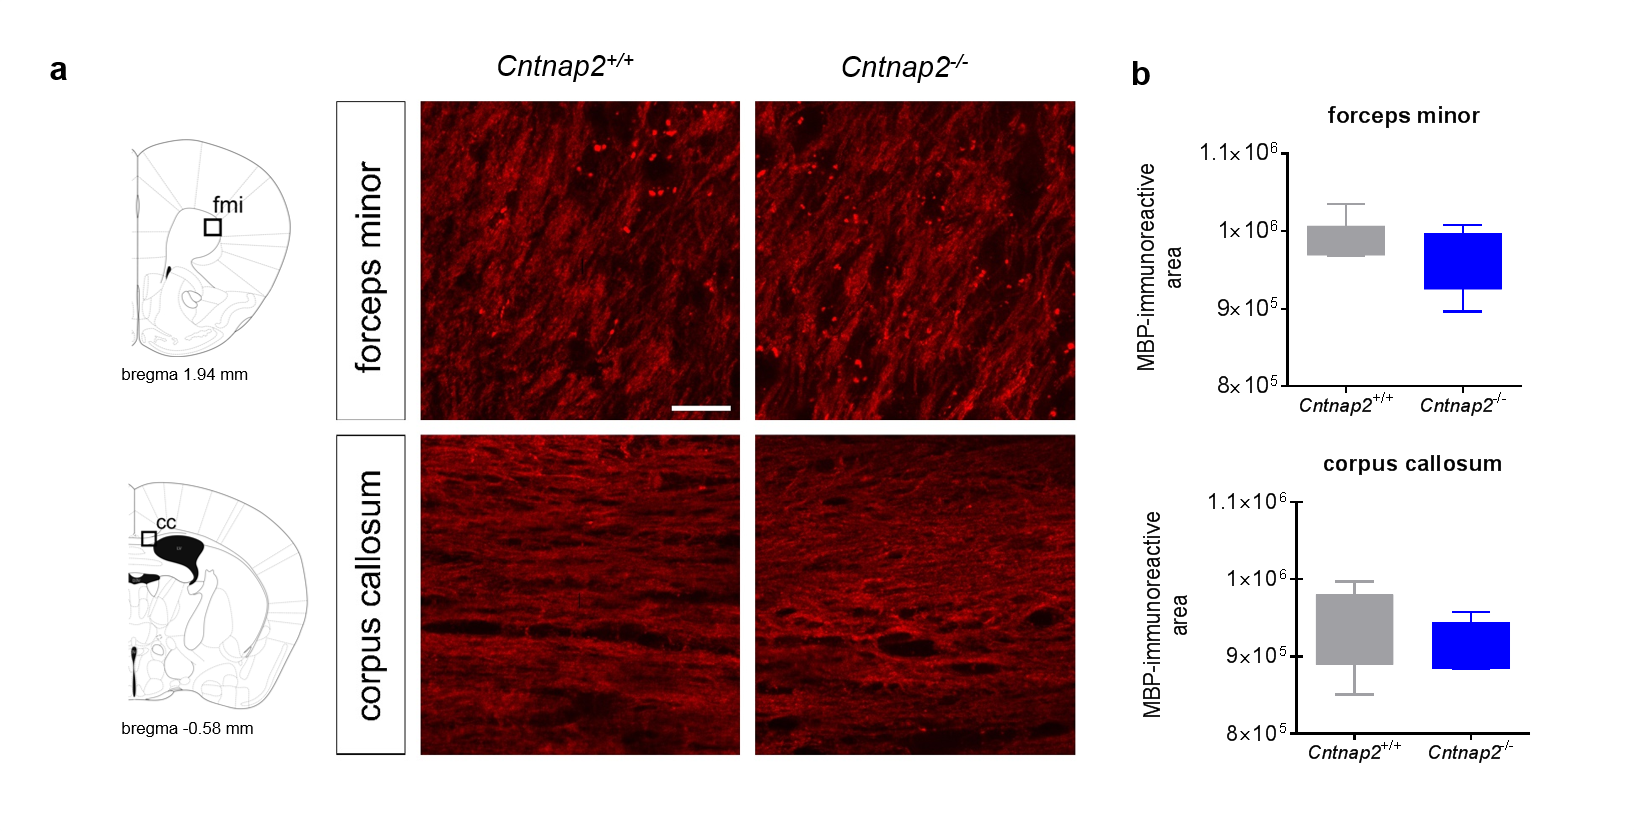
\includegraphics[scale=0.5]{figures/cntnap2_figure_s8.png}
    \decoRule
    \caption[Histological and immunohistochemical analysis of white
    matter.]{Histological and immunohistochemical analysis of white matter.
    (\textbf{a}) Representative images of anterior callosal regions
    characterized by parallel or transversal fibre extension with respect to the
    imaging plane (corpus callosum and forceps minor of the corpus callosum,
    respectively). No apparent difference in fibre organization or MBP stained
    regions was observed between genotypes. (\textbf{b}) MBP-immunoreactive area
    averaged from three random image fields per region and animal (n = 5, each
    group; corpus callosum: t-test, t8 = 0.84, p = 0.42; forceps minor of the
    corpus callosum: t-test, t8 = 1.06, p = 0.32).}
    \label{fig:cntnap2_figs8}
\end{figure}

\section{Discussion}

Here we show that homozygous mice lacking \textit{Cntnap2}, a neurexin superfamily member
associated with autism, exhibit reduced long-range and local functional
connectivity in prefrontal cortical regions and midline functional hubs of the
mouse brain, an effect that may involve defective cingulate-prefrontal mesoscale
wiring. We also show that reduced fronto-posterior connectivity is associated
with impaired social behaviour, revealing a possible link between long-range
functional connectivity alterations and mouse behavioural traits recapitulating
ASD symptoms. Collectively, these findings suggest that loss-of-function
mutations in \textit{Cntnap2} may predispose to neurodevelopmental disorders and autism
through dysregulation of macroscale functional network couplings.

Our use of an imaging readout widely employed in human connectivity mapping
provides us with the opportunity to cross-compare connectivity findings across
species. In this respect, the observation of long-range fronto-posterior
hypo-connectivity in \textit{Cntnap2}$^{-/-}$ mice is especially noteworthy, because it is in
excellent agreement with the results of a recent human imaging study where an
association between common genetic variants in CNTNAP2 and similar long-range
frontal hypoconnectivity was described \parencite{scott-vanzeeland2010}. Our
results expand these findings, by revealing a causal contribution of \textit{Cntnap2}
loss-of-function mutations to long-range fronto-cortical connectivity
impairments. These correspondences also serve as an important proof-of-concept
demonstration that ASD-related genetic mutations can lead to comparable
macroscale connectivity deficits in humans and lower mammal species like the
laboratory mouse. The presence of long-range hypoconnectivity in \textit{Cntnap2}$^{-/-}$ mice
also adds to the remarkable construct and face validity of this mouse model as
an experimental tool for mechanistic and therapeutic investigation of syndromic
forms of ASD \parencite{penagarikano2011}. Specifically, \textit{Cntnap2}$^{-/-}$ mice closely
recapitulate major neuropathological features observed in cortical
dysplasia-focal epilepsy (CDFE) syndrome, a rare neuronal migration disorder
associated with a recessive (suggesting loss of function) mutation in CNTNAP2,
and, in nearly two thirds of patients, with autism \parencite{strauss2006}.
These include behavioural deficits in the three core domains of ASD (reduced
vocal communication, repetitive and restricted behaviours, and abnormal social
interactions), hyperactivity and epileptic seizures (both features described in
CDFE patients), and reduced GABAergic interneurons, resulting in asynchronous
cortical activity as measured with in vivo two-photon calcium imaging
\parencite{penagarikano2011}.

The observation of defective mesoscale axonal wiring in the cingulate cortex
corroborates the presence of selective prefrontal dysregulation in \textit{Cntnap2}$^{-/-}$
mutants, and serves as a possible neuroanatomical correlate for some of the
prefrontal functional connectivity impairments mapped with rsfMRI. Regional
differences in GABAergic interneuron density, and developmental processes
related to circuit and network refinements \parencite{zhan2014, riccomagno2015}
are, however, likely to play a role in the observed functional desynchronization
as well, given the established contribution of GABAergic oscillatory rhythms in
mediating large-scale functional synchrony \parencite{gonzalez-burgos2008} and
the recent evidence of altered spine density and increased spine eliminations in
\textit{Cntnap2}$^{-/-}$ mice \parencite{gdalyahu2015}. The relative contribution of
anatomical versus neurophysiological mechanisms in determining the observed
desynchronization remains however undetermined, and interventional studies
entailing the regional manipulation of excitatory/inhibitory ratio or
inactivation of projection-specific pathways may be required to disambiguate
this issue.

Recent human studies described possible microstructural white matter
alterations in carriers of CNTNAP2 mutations as assessed with water diffusion
anisotropy.  Specifically, gender-dependent reductions in fractional anisotropy
(FA) in the inferior fronto-occipital fasciculus or anterior thalamic radiation
have been described by \textcite{tan2010}. Similarly,
\textcite{clemmvonhohenberg2013} described an interaction between a single
genotype (rs2710126) and FA, in which homozygotes for the risk allele showed
reduced FA values in uncinate fasciculus. 

These preliminary results suggest the presence of possible white matter
microstructural alterations as a result of CNTNAP2 gene mutations. However,
anisotropic water diffusion reflects multiples biophysical contributions that
prevent an unequivocal microstructural interpretation of these findings. For
example, reduced FA could be the result of reduced neuronal packing,
myelinisation, axonal diameter, neuronal integrity and maturation, as well as
regional differences in gray matter fraction \parencite{beaulieu2009}. To
investigate potential microstructural white matter disruption at a more detailed
level than permitted by diffusion MRI, we carried out a histological assessment
of white matter fibres using MBP immunofluorescence. We did not observe any
gross white matter microstructural abnormality in \textit{Cntnap2}$^{-/-}$ mutants in terms of
fibre orientation, packing or organization. Moreover, MBP quantification did not
reveal any significant genotype-dependent differences. Together with previous
electron microscopy investigations, where normal myelin thickness was reported
in \textit{Cntnap2}$^{-/-}$ mutants \parencite{poliak2003}, these findings argue against the
presence of gross microscale white matter alterations in these mutants. While
this finding appears to be in contrast with human investigations of CNTNAP2
polymorphisms and suggestive of possible species-specific divergence, additional
research is required to more thoroughly investigate the presence of white matter
microstructural aberrancies in \textit{Cntnap2}$^{-/-}$ mutants. It should also be noted that
CNTNAP2 polymorphisms studies in humans are typically correlative and involve
small patient samples, which make them more prone to confounding factors related
to heterogeneity in clinical samples, and individual adaptive differences in
microstructural parameters \parencite{scholz2009}.

The observation of hypoconnectivity in prefrontal hub regions of the DMN
\parencite{liska2015} is suggestive of a deficient “maturation” of this
functional network (supekar2010), and is in keeping with the hypothesis of a key
role of this region as a mediator of deficits in global perception and its
cognitive representations in ASD patients \parencite{martinez-sanchis2014}. The
notion that “underconnectivity” may preferentially affect complex cognitive and
social functions and their high order cortical substrates rather than low-level
sensory and perceptual tasks has recently found some theoretical support
\parencite{kana2011}.  Within this framework, heteromodal integrative hubs like
the anterior cingulate and prefrontal cortex, as well as retrosplenial regions
would serve as major points of vulnerability for the stability of distributed
functional network couplings. rsfMRI mapping in additional mouse lines
harbouring ASD-related genetic mutations will be instrumental in assessing
whether the observed alterations represent a generalizable endophenotype that
may converge across mutations and genetic etiologies, or are the specific
consequence of \textit{Cntnap2} mutations. It is, however, interesting to note that so
far hypoconnectivity appears to be predominant in mouse imaging studies of ASD:
reduced connectivity in several brain regions including the prefrontal cortex
and the DMN has been observed in the BTBR model of idiopathic autism
\parencite{sforazzini2016}, and in mice characterised by reduced synaptic
pruning \parencite{zhan2014}, a pathological trait associated with autism
\parencite{tang2014}. Reduced connectivity between motor sensory regions and a
general reduction in primary visual cortex connectivity were also recently
described in a mouse model of fragile X syndrome (haberl2015). Although
preliminary, these initial mouse findings are consistent with and somehow
support the “under-connectivity theory” of autism, according to which reduced
functional connectivity, at least in the adult brain \parencite{uddin2013}, may
emerge as a dominant feature of ASD in the face of heterogeneous
etiopathological pathways \parencite{dimartino2014a, uddin2013}.

In contrast with our imaging results, human rsfMRI mapping in CNTNAP2 common
variant carriers revealed increased, instead of decreased, local connectivity in
lateral prefrontal regions (scott-van2010). The reason behind this discrepancy
is not clear, although several important experimental factors, including
methodological, species- and/or age-related differences may contribute to this
inconsistency. For example, local connectivity was found to be increased in
human lateral prefrontal areas, a region that does not have a clear
cyto-architectural correlate in rodents \parencite{vogt2014}. Moreover, our
study was performed in adult male subjects, while human mapping was carried out
in pre-pubertal subjects (mean age 12 years old), a discrepancy that could
account for the differences in local connectivity alterations. Indeed, a
dramatic reorganization of large-scale functional brain networks occurs during
childhood and late adolescence in humans, involving developmental shifts from
short-range to long-range connectivity, notably within fronto-insular and
cortico-subcortical networks [reviewed by \parencite{ernst2015}]. Moreover, an
age-related dichotomy has been suggested in ASD-related connectivity
aberrancies, with generally reduced intrinsic functional connectivity in
adolescents and adults with autism compared with age-matched controls, and
increased functional connectivity in younger children with the disorder
\parencite{uddin2013}. A similar age-related shift could therefore possibly
explain the discrepant direction of local connectivity observed in our study
with respect to the finding reported by \textcite{scott-vanzeeland2010} in
human pre-adolescent subjects. Longitudinal investigations of connectivity in
rodent genetic models of autism are highly warranted to enable empirical testing
of the developmental trajectory of ASD-related connectivity aberrancies across
development and network maturation \parencite{liska2016}. Finally, differences
in the nature of the investigated mutations should also not be neglected, as
the functional consequences of the genetic variants imaged by
\textcite{scott-vanzeeland2010} are unclear, and the possibility that not all
the imaged genetic variants are loss-of-function cannot be ruled out. 

We also note here that our study specifically addressed male mice only, owing to
the greater ASD incidence in this gender \parencite{lai2015}. While this choice
has the advantage of reducing within-group variation and subsequent increase in
statistical power of our measurements, this should be considered a limitation of
our study, as it does not permit to assess whether our findings can be
generalized to female carriers of \textit{Cntnap2} loss-of-function mutations. 

In conclusion, we document that the absence of \textit{Cntnap2} leads to functional
connectivity reductions and defective mesoscale wiring in prefrontal functional
hubs of the mouse brain, an effect associated with impaired social behaviour.
These findings suggest that loss-of-function mutations in \textit{Cntnap2} may predispose
to neurodevelopmental disorders and autism through selective dysregulation of
connectivity in integrative prefrontal areas, and provide a translational model
for investigating connectional perturbations in syndromic ASD forms.
